\documentclass{article}

\usepackage{amssymb,amsmath}
\usepackage{graphicx}
\usepackage{floatflt}
\usepackage[left=1in,top=1in,right=1in]{geometry}
\usepackage{xr}
\usepackage{xr-hyper}
\usepackage{hyperref}
\usepackage{longtable}

\hypersetup{
    bookmarks=true,         % show bookmarks bar?
    unicode=false,          % non-Latin characters in Acrobat�s bookmarks
    pdfnewwindow=true,
    pdfborder={0 0 0 0},
    pdftoolbar=true,        % show Acrobat�s toolbar?
    pdfmenubar=true,        % show Acrobat�s menu?
    pdffitwindow=true,      % page fit to window when opened
    pdftitle={High Level Design},    % title
    pdfauthor={Andrew Atutis, Joe Belmont, Steve Deyo, Ryan Edgar, Jon Eggleston, John Ellis, Jacor Finlayson, Michael Hadley, James Licata, Brett Peplowski},     % author
    pdfsubject={EE418: Software Engineering Senior Design},   % subject of the document
    pdfkeywords={keywords}, % list of keywords
    colorlinks=false       % false: boxed links; true: colored links
}


\externaldocument{system_requirement_specification}


\title{High Level Design}
\author{Andrew Atutis \and Joe Belmont \and Steve Deyo \and Ryan Edgar \and Jon Eggleston \and John Ellis \and Jacor Finlayson \and Michael Hadley \and James Licata \and Brett Peplowski}
\date{\today}


\setcounter{tocdepth}{3}

\begin{document}

\begin{titlepage}
\maketitle
\end{titlepage}


\tableofcontents

\newpage

\section{Introduction}
This document states the high level design for the Mobile Pedometer system. This document should be used by the designers and developers as a basis for the implementation of the system, as it also contains system level use cases, and state diagrams.  The goal of this high level design document is to make the reader knowledgeable on the structural design of the system, as well as more knowledgeable about what the system does/is capable of doing.
The Activity Monitor system will provide a better way to monitor patient rehabilitation using a Wii Remote and a PDA (Palm Treo 750). The system will be targeted towards nursing homes and rehab hospitals which require monitoring of elderly people, recovering athletes, and people with balance issues. The system will further provide independent mobility while monitoring a patients progress with prescribed Daily Tasks. 
To perform this, we have developed a Web UI, complete with a database application, which is easy to use and can safely and securely store a patients data.

\newpage

\section{Use Cases}
The diagram below shows all of the interactions each user will be able to do with the system once they log in or power on. Patients will interact with the PDA, while Researchers and Clinicians interact with the Web UI.
All patients have the ability to start the PDA application, begin their daily task, upload data to the server, and complete their daily task.
Researchers and Clinicians share many uses of the system, including Viewing Patient Health Charts, Logging into the Web UI, and Viewing Patient Completion Charts. The Clinician has some accesses to the system that a Researcher does not however. The Clinician may Add Patients to the Web UI as well as assign Daily Tasks.
Researchers may view Group Patient Health Charts to compile trends.


\begin{center}
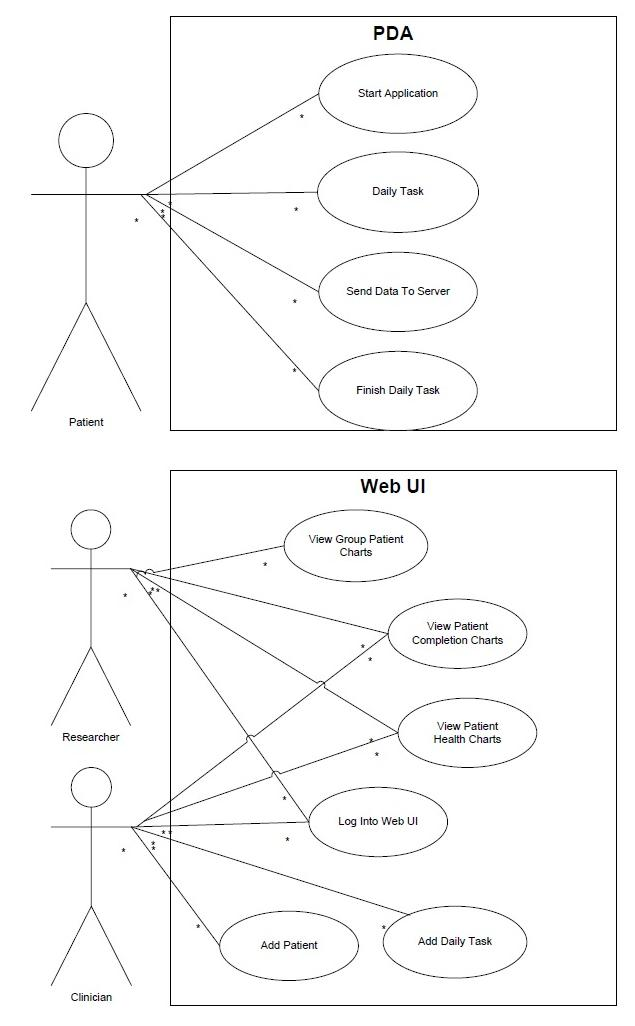
\includegraphics[width=4in, height=6.46in]{HLDuseCaseDiagram.jpg}
\label{fig:usecase}
\end{center}


\section{Scenarios}
The following describe common paths that a user may take through the system.

\subsection{Patient goes through their Daily Task}	
The system will provide the following features:
\begin{enumerate}
\item The Patient starts the Activity Monitor application on the PDA.
\item The PDA begins to monitor walking activity. 
\item The Patient completes the Daily Task and is presented with an alert on the PDA. 
\item The PDA begins to download the computed PDA Statistics to the server. The PDA also updates the Daily Task for the next day. 
\item The patient exits the Activity Monitor application.
\end{enumerate} 

\subsection{Clinician adds a new patient}	
The system will provide the following features:
\begin{enumerate}
\item A Clinician logs onto the web interface.
\item The Clinician navigates to the Add Patient page.
\item The Clinician enters the relevant Patient Profile information.
\item The Clinician submits the form and the Patient is added to the database.
\item The Clinician logs off the Web UI.
\item The Clinician configures the PDA so that it will log in the patient with their unique Username and Password.
\end{enumerate} 

\subsection{A Clinician adds a new task for a patient}	
The system will provide the following features:
\begin{enumerate}
\item A Clinician logs onto the Web UI
\item The Clinician navigates to the List Patients page.
\item The Clinician then clicks on the appropriate Patient and the Patients profile information is displayed.
\item The Clinician clicks on the New Daily Task button.
\item The Clinician enters the appropriate data.
\item The Clinician logs off the Web UI.
\end{enumerate} 

\subsection{A Clinician reviews Patient Completion Charts/Patient Health Charts}	
The system will provide the following features:
\begin{enumerate}
\item A Clinician logs onto the Web UI
\item The Clinician navigates to the List Patients page.
\item The Clinician clicks on the appropriate Patient.
\item The Clinician clicks on the Patient Health Chart or the Patient Completion Chart
\item The correct chart is displayed with the correct statistical data.
\item The Clinician analyzes the data and discusses with the Patient.
\item The Clinician logs off the Web UI.
\end{enumerate} 

\subsection{A Researcher reviews Patient Completion Charts/Patient Health Charts/Group Patient Charts}	
The system will provide the following features:
\begin{enumerate}
\item A Researcher logs onto the Web UI
\item The Researcher navigates to the Patient Completion Chart/Patient Health Chart/Group Patient Chart.
\item The Researcher analyzes the data and reports back to the appropriate Clinicians.
\item The Researcher logs off the Web UI.
\end{enumerate} 



\newpage
\section{System Flow}
The following diagram shows how the overall system will function.


\begin{center}
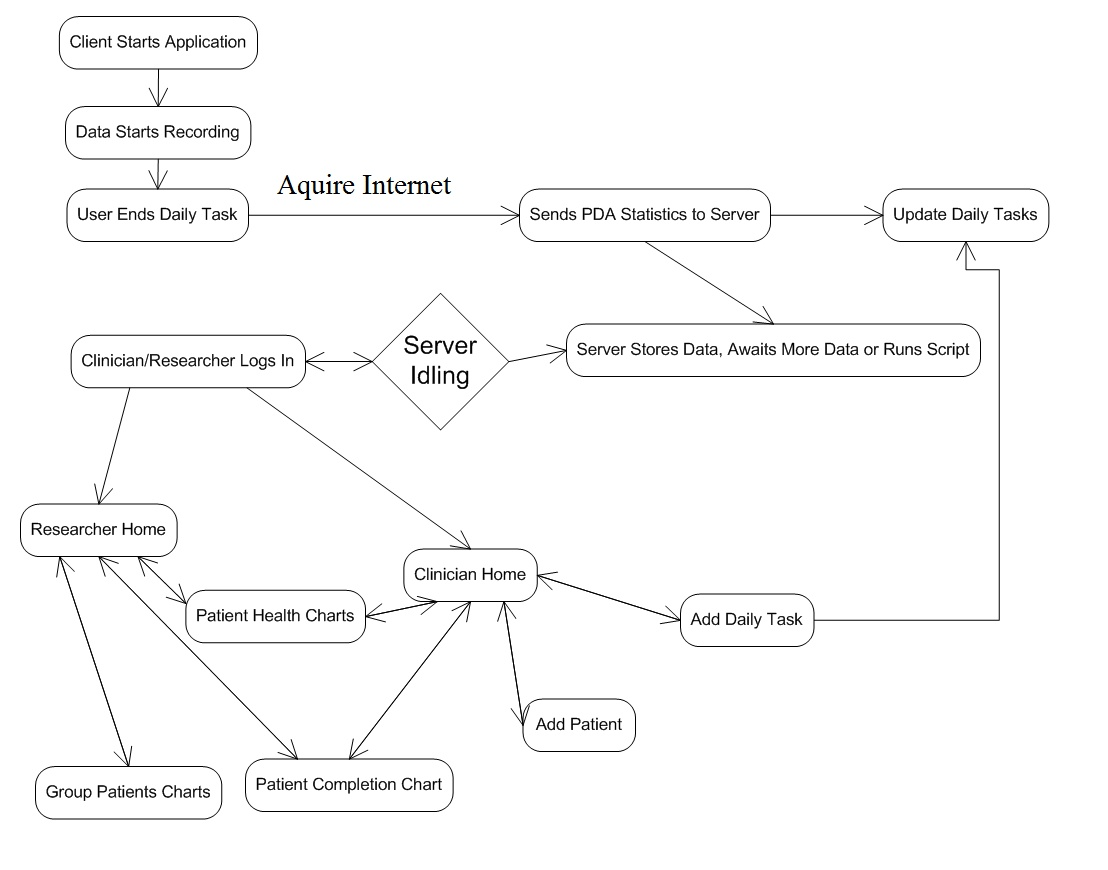
\includegraphics[width=6in, height=5in]{HLDSystemFlow.jpg}
\label{fig:systemflow}
\end{center}


\newpage

\section{User Flow}
The following diagram shows the paths for the user interface.

\begin{center}
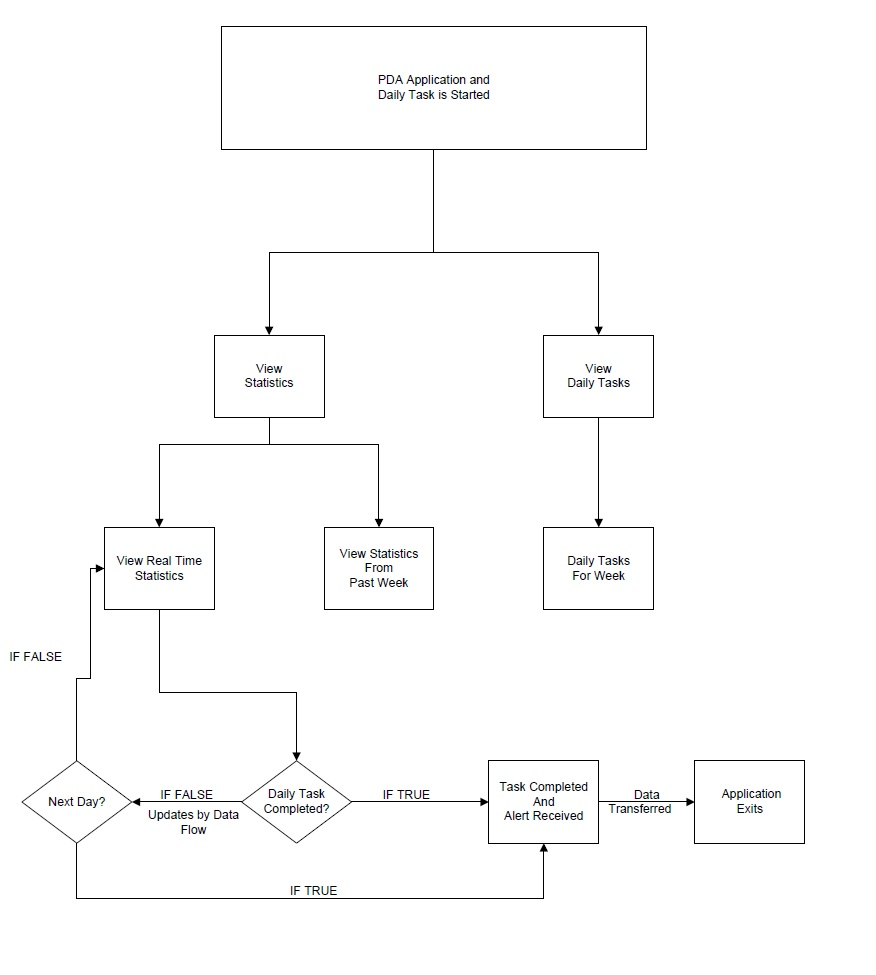
\includegraphics[width=6in, height=6.67in]{HLDuserFlow.jpg}
\label{fig:userflow}
\end{center}


\newpage

\section{Data Flow}
The following shows the data flow through the application and server.

\begin{center}
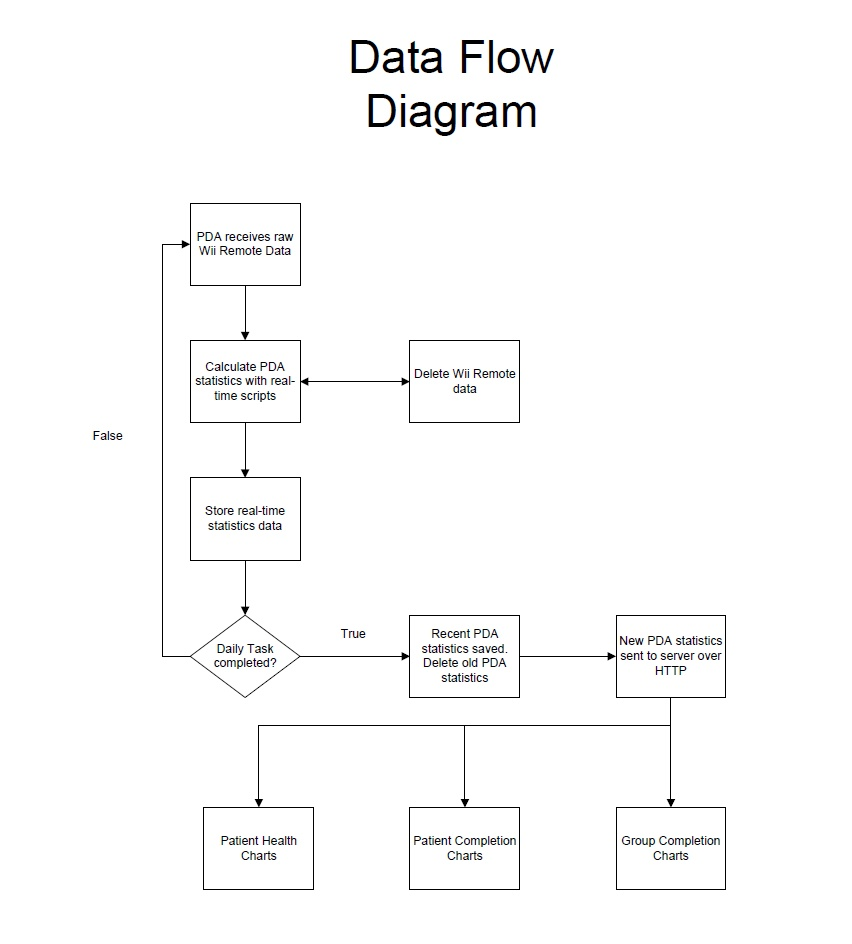
\includegraphics[width=6in, height=6.5in]{HLDdataFlowDiagram.jpg}
\label{fig:dataflow}
\end{center}

\newpage

\section{Major System Components}

The follow details the major components of the Activity Monitor system. For a illustration see Figure \ref{fig: Major System Components}: \nameref{fig: Major System Components}

\begin{figure}[p]
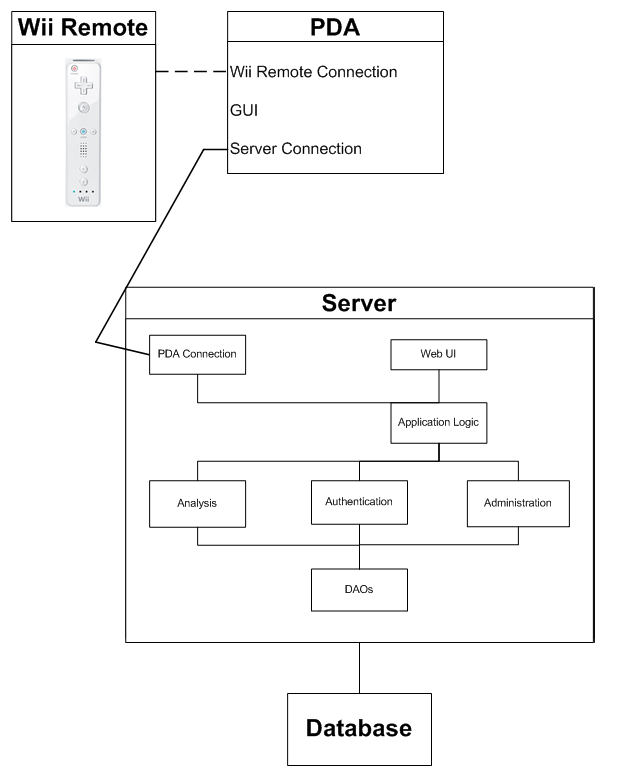
\includegraphics[width=6in,height=7.44in]{major_system_components.png}
\caption{Major System Components Diagram}
\label{fig: Major System Components}
\end{figure}

\subsection{PDA}

\paragraph{Client GUI}

\paragraph{Wii Remote Connection}
This component represents the software entity that will reside on the PDA. It is responsible for establish a Bluetooth connection with the Wii Remote and retrieving the Raw Wii Remote Data.

\paragraph{Server Connection}
This component represents the software entity residing on the PDA which will authenticate with the server, and transmit PDA Statistics to the server. This component will also manage updates to the Patient's Daily Tasks.

\subsection{Server}

\paragraph{PDA Connection}
This component will reside on the Server and will be responsible for managing the transfer of data to and from the PDA. This component will talk to the Server Connection component on the PDA. These two entities will performing a handshaking protocol (during authentication) as well as transmit PDA Statistics and Daily Task updates.

\paragraph{Web User Interface}
This component will represent the software component that encompasses the three-tiered Web Application which will reside on the Server. The Web UI will contain a Client User Interface, Application Logic, and a Database.

\paragraph{Application Logic}
This software entity will fit between the Client User Interface and the Database. It will process Client requests and access the appropriate information from the Database. 

\subparagraph{Analysis}
This entity will be contained in the Application Logic. It will deal with processing Client requests pertaining to Clinician and Researcher Charts. The module will retrieve the appropriate information from the Database in order to present the requested chart to the Clinician or Researcher.

\subparagraph{Authentication}
This entity will be contained in the Application Logic. It will deal with processing Researcher/Clinician/Patient Login information. It will verify each user's credentials and report back an appropriate message to the user.

\subparagraph{Administration}
This entity will be contained in the Application Logic and will deal primarily with Adding/Removing/Editing Clinicians, Researchers, and Patients, Modifying Daily Tasks, and shifting Patients between Clinicians.

\subparagraph{Database Access Objects (DAOs)}
This entities will be used to directly modify the Database Object Models. This represents the final stage of the Application Logic and provides an avenue to actually access the Database. 

\newpage

\section{Object Oriented Domain Analysis}

\subsection{Common Object Architecture}\label{sec: common objects}

\begin{center}
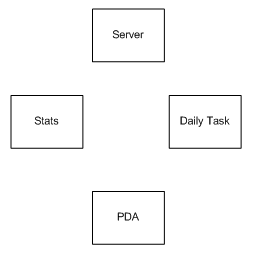
\includegraphics{Server3_ooda.png}
\end{center}

\paragraph{DailyTask}
\subparagraph{Description}
This object represents the patient's daily task.  The object is known to both the Server and the PDA.  This allows both system components to perform operations and access the daily task.  The daily task object can represent in theory a wide variety of activities. The simplest being to walk a predetermined number of steps.  The Server to PDA interface provides a means of transfer the data associated with a daily task object from the Server to the PDA. 
\subparagraph{Requirements}
\begin{itemize}
\item \nameref{sec: Mod Daily Task}
\item \nameref{sec: PDA Update Task}
\item \nameref{sec: View Task}
\end{itemize}

\paragraph{Stats}\label{sec: Stats Obj}
\subparagraph{Description}
The Stats object is associated with a given sampling period, over which certain statistics are computed by the PDA. The object is known to both the PDA and the Server which allows the statistics to be transferred from the PDA to the Server. This will facilitate organization of the collected data within the database on the Server. It also provides an irreducible unit of sampling time of which the graphs and charts can be constructed.
\subparagraph{Requirements}
\begin{itemize}
\item \nameref{sec: PDA Displays Stats}
\item \nameref{sec: Health Chart}
\item \nameref{sec: Group Chart}
\item \nameref{sec: Completion Chart}
\end{itemize}

\newpage
\subsection{PDA Object Architecture}

\begin{center}
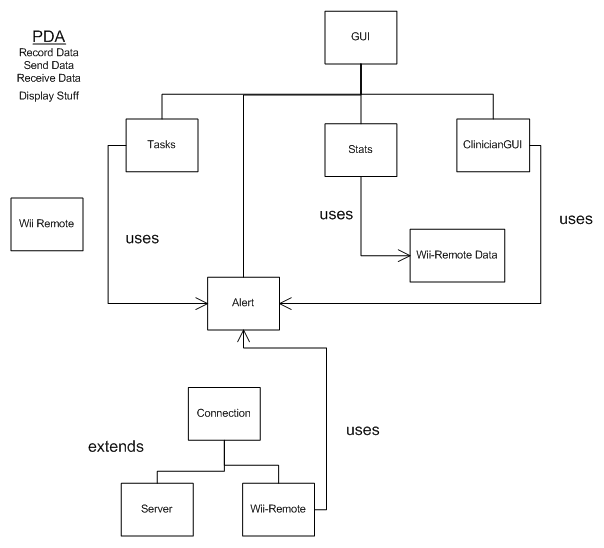
\includegraphics[width=6in,height=5.45in]{PDA_ooda.png}
\end{center}

\subsubsection{Wii Remote Handling}
\paragraph{Connection}
The Connection object provides an interface for the PDA to establish connection with the Wii-Remote and determine the status of the Wii-Remote.
\paragraph{WiiRemote}
\subparagraph{Description}
This object encompasses all interaction with the Wii-Remote. This includes connection, and the data obtained from the Wii-Remote. 
\subparagraph{Requirements}
\begin{itemize}
\item \nameref{sec: PDA Wii Conn}
\item \nameref{sec: Conn Mode}
\item \nameref{sec: Wii Conn Lost}
\item \nameref{sec: Battery Status}
\item \nameref{sec: Wii Vibrate}
\end{itemize}

\paragraph{WiiRemoteData}
\subparagraph{Description}
The WiiRemoteData object provides an interface to receive and interpret data from the Wii-Remote to the PDA.
\subparagraph{Requirements}
\begin{itemize}
\item \nameref{sec: PDA Records Data}
\item \nameref{sec: PDA Displays Stats}
\end{itemize}

\subsubsection{Server Connection Handling}
\paragraph{Connection}
\paragraph{ServerConnection}
\subparagraph{Description}
The ServerConnection object provides an interface for the PDA to connect with the Server to send and receive data. Data that has been collected by the PDA from the WiiRemote will be sent to the Server, while the PDA will update the Patients Daily Task according to the Servers data being sent back to the PDA.
\subparagraph{Requirements}
\begin{itemize}
\item \nameref{sec: Data Dump}
\item \nameref{sec: Emer Data Dump}
\item \nameref{sec: PDA Server Conn}
\item \nameref{sec: PDA Update Task}
\end{itemize}

\paragraph{Stats}
This is a shared object between the PDA and the Server architectures. For more information see Section \ref{sec: common objects}: \nameref{sec: common objects}.

\paragraph{DailyTask}
This is a shared object between the PDA and the Server architectures. For more information see Section \ref{sec: common objects}: \nameref{sec: common objects}.


\subsubsection{Client General User Interface}
\paragraph{StatsView}
\subparagraph{Description}
The StatsView object interprets Alert Messages for when the Daily Task is completed and displays them to the user, while also displaying real time PDA statistics to the user.
\subparagraph{Requirements}
\begin{itemize}
\item \nameref{sec: Task Completed}
\item \nameref{sec: PDA Displays Stats}
\end{itemize}
\paragraph{DailyTaskView}
\subparagraph{Description}
The DailyTaskView object displays Daily Tasks to the user as interpreted from the data collected from the server in easy to read font on the PDAs display.
\subparagraph{Requirements}
\begin{itemize}
\item \nameref{sec: View Task}
\item \nameref{sec: Large Font}
\end{itemize}
\paragraph{ClinicianGUI}
\subparagraph{Description}
The ClinicianGUI object provides an interface for the clinician to enter the information required to connect to the server. This includes the server address, the patient's username, and the patient's password. The information entered on this screen is known only to the clinician. Access to this screen should be obscured from the patient's general activities on the PDA.
\subparagraph{Requirements}
\begin{itemize}
\item \nameref{sec: PDA Server Conn}
\end{itemize}
\paragraph{Alert}
\subparagraph{Description}
This object will deal with all the alerts provided to the Patient on the PDA. This includes alerts for when the Patient completes an exercise, a connection is lost between the PDA and the Wii Remote, and when the PDA goes into Emergency Data Dump Mode. 
\subparagraph{Requirements}
\begin{itemize}
\item \nameref{sec: Emer Data Dump}
\item \nameref{sec: Alerts}
\item \nameref{sec: Wii Conn Lost}
\item \nameref{sec: Battery Status}
\item \nameref{sec: Task Completed}
\end{itemize}

\newpage
\subsection{Server Object Architecture}

\begin{center}
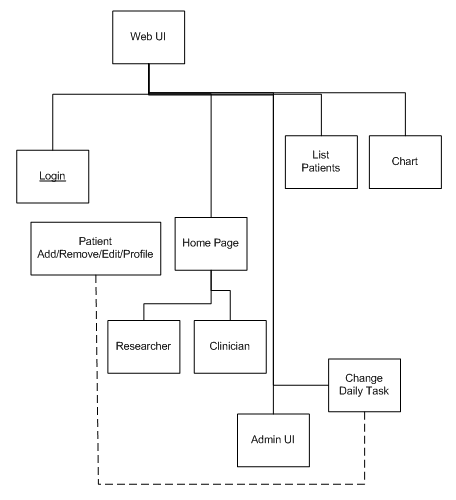
\includegraphics[width=4.75in,height=5.21in]{Server1_ooda.png}\label{fig: webui}
\end{center}

\begin{center}
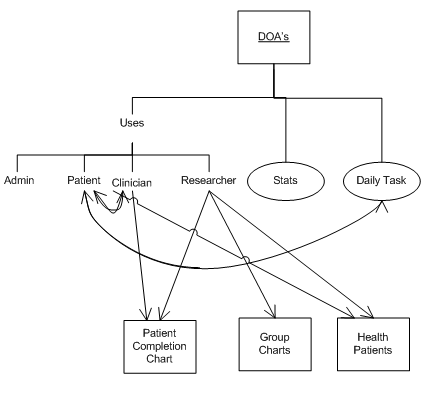
\includegraphics[width=4.56in,height=4.09in]{Server2_ooda.png}
\end{center}

\subsubsection{PDA Interaction}

\paragraph{Server}
\subparagraph{Description}
This is the primary control object on the server side. It will maintain interactions with multiple PDAs and handle any and all administrative and authentication related issues.

\paragraph{PDA}
\subparagraph{Description}
This object represents all interaction with the PDA from the Server. It encompasses all of the connection interfaces, as well as PDA Statistics data exchange, and the front-end GUI portion. 
\subparagraph{Requirements}
\begin{itemize}
\item \nameref{sec: Data Dump}
\item \nameref{sec: Emer Data Dump}
\item \nameref{sec: PDA Server Conn}
\item \nameref{sec: PDA Update Task}
\end{itemize}

\paragraph{Stats}
This is a shared object between the PDA and the Server architectures. For more information see Section \ref{sec: common objects}: \nameref{sec: common objects}.

\paragraph{DailyTask}
This is a shared object between the PDA and the Server architectures. For more information see Section \ref{sec: common objects}: \nameref{sec: common objects}.

\subsubsection{Web User Interface}

This directly fulfills the requirement: \nameref{sec: Web UI}. 

\paragraph{Login}
\subparagraph{Description}
This object represents all of the logins on the Web UI by both Clinicians and Researchers. It is responsible for querying the Application Logic's Authentication module for verification of the user's credentials. 
\subparagraph{Requirements}
\begin{itemize}
\item \nameref{sec: Researcher Login}
\end{itemize}

\paragraph{PatientProfile}
\subparagraph{Description}
This object represents a Patient's account in the Web UI. This object has a many to one relationship with Clinicians. It contains all of the relevant Patient information, as well as a Username and Password for the PDA.
\subparagraph{Requirements}
\begin{itemize}
\item \nameref{sec: Patient Profile}
\item \nameref{sec: Unique Usernames}
\item \nameref{sec: List Patients}
\end{itemize}

\paragraph{HomePage}
\paragraph{ResearcherHome}
\paragraph{ClinicianHome}
\paragraph{AdminUI}
\subparagraph{Description}
This object will represent the user interface presented to the Administrator in order to Add or Remove Researcher and Clinician user accounts in the Web UI.
\subparagraph{Requirements}
\begin{itemize}
\item \nameref{sec: Administrator Add/Remote/Edit}
\item \nameref{sec: Unique Usernames}
\item \nameref{sec: Administrator Homepage}
\end{itemize}

\paragraph{ChangeDailyTask}
\subparagraph{Description}
This object is responsible for changes to a specific Patient's Daily Tasks. It will query the Web UI's Application Logic unit's Administration module to modify the database. 
\subparagraph{Requirements}
\begin{itemize}
\item \nameref{sec: Mod Daily Task}
\end{itemize}

\paragraph{ListPatients}
\subparagraph{Description}
This object will be accessible to users through the web user interface. It should provide a list of available patients for the currently logged in user as a web page output. This list must include only patients that are under the control of the clinician logged in. Security on this page is of the utmost concern.

The page generated by this object should be simple to understand and easy to navigate. The patient listing that is generated should provide links to each patient's profile. 

\subparagraph{Requirements}
\begin{itemize}
\item \nameref{sec: Patient Profile}
\item \nameref{sec: List Patients}
\end{itemize}

\paragraph{Chart}
\subparagraph{Description}
This object will be an abstract base for the Researcher and Clinician Charts.
\subparagraph{Requirements}
\begin{itemize}
\item \nameref{sec: Health Chart}
\item \nameref{sec: Group Chart}
\item \nameref{sec: Completion Chart}
\end{itemize}
\paragraph{CompletionChart}
\subparagraph{Description}
This chart is available to both Clinicians and Researchers and represents a if particular Patient is completing their Daily Tasks. 
\subparagraph{Requirements}
\begin{itemize}
\item \nameref{sec: Completion Chart}
\end{itemize}
\paragraph{HealthChart}
\subparagraph{Description}
This chart is available to both Clinicians and Researchers and represents how a particular Patient's Health has improved over the course of their treatment.
\subparagraph{Requirements}
\begin{itemize}
\item \nameref{sec: Health Chart}
\end{itemize}
\paragraph{GroupChart}.
\subparagraph{Description}
This chart is only available to the Researcher and represents trends pertaining to groups of Patient's Daily Tasks. 
\subparagraph{Requirements}
\begin{itemize}
\item \nameref{sec: Group Chart}
\end{itemize}


\section{Object Interface Specification}

\subsection{PDA to Server Interfaces}
\begin{center}
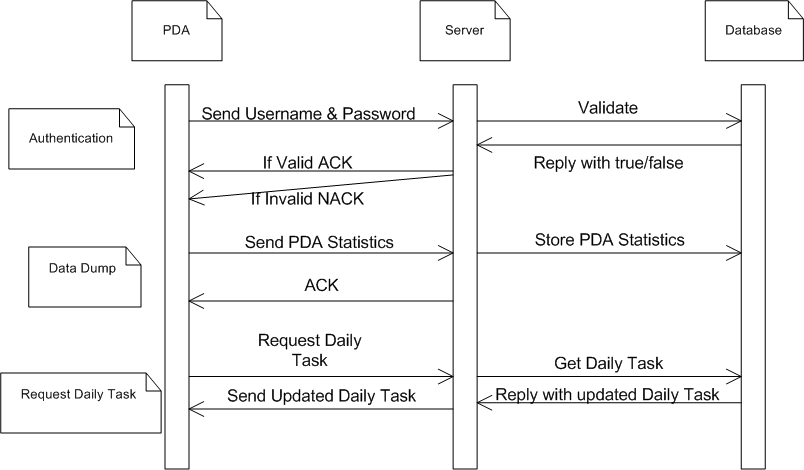
\includegraphics{PDA_to_Server_Interface_Diagram.png}
\end{center}

\paragraph{Authentication}
\subparagraph{Description}
The main purpose of the authentication is to verify that the correct user is trying to access the patients information. At the authentication screen, the user will enter their username and password. The username and password that was entered is sent to the server. If the information is correct ACK is sent back by the server. If not, NACK is sent back, and the connection is closed. Once the information is verified, the validation is sent to from the server to the database. 
\subparagraph{Trigger}
This task occurs when the PDA is handshaking with the Server during the initialization of a connection. This connection could either be triggered by the need to download the daily task or the need to dump data to the server.

\paragraph{Data Dump}
\subparagraph{Description} 
The data dump is used to send the information stored on the PDA for the day to the database. At the end of the day, the data is sent over an open connection to the server. When the server receives the information, an ACK is sent back. Once this is done, the information is sent from the server and stored into the database. 
\subparagraph{Trigger}
The data dump task is triggered by the completion of a day. The actual data dump request occurs after authentication with the Server.

\paragraph{Request Daily Task}
\subparagraph{Description}
The user must be able to request a daily task from the database. At the beginning of the day, or while a data dump is occurring, the user sends the request to the server. When this request is received by the server, the server will search through the database to retrieve the tasks for the specified users. When the tasks are found, they are sent back to the PDA, allowing the user to view them. 
\subparagraph{Trigger}
The request daily task event occurs before the beginning of a new day or during a data dump connection. The actual request is sent after authentication with the Server.

\subsection{Web UI Interfaces}

\begin{center}
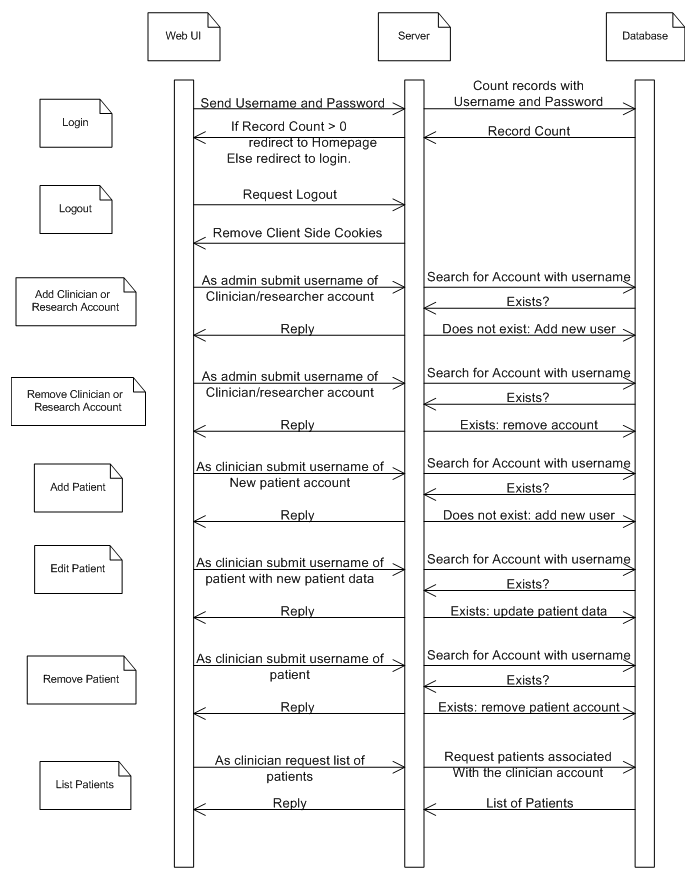
\includegraphics[width=6in,height=7.44in]{webui_interfaces_1.png}
\newpage
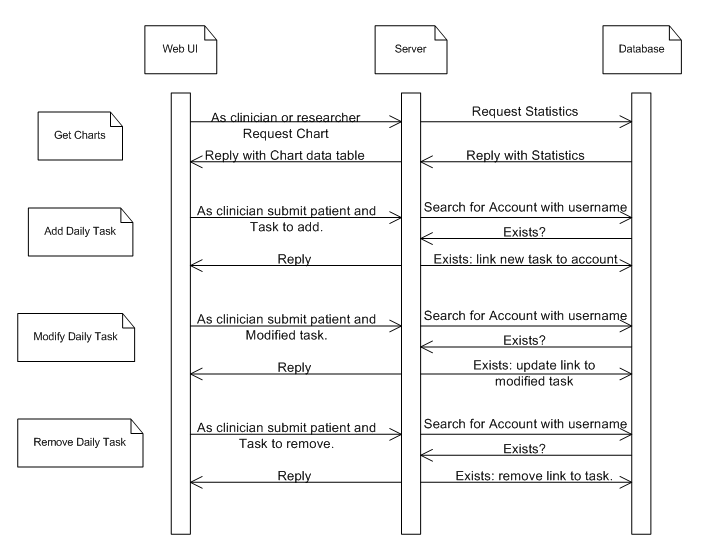
\includegraphics[width=6in,height=4.72in]{webui_interfaces_2.png}
\end{center}

\paragraph{Login}
\subparagraph{Description}
The clinician or researcher is attempting to access the privileged material available within the Web UI. In order to access this material the clinician or researcher must be a registered user of the system.
\subparagraph{Trigger}
A request is made to the Web UI to login an account with the provided username and password. Generally this request is generated by a web browser when the client clicks the ``Login'' button on the login web page.

\paragraph{Logout}
\subparagraph{Description}
The task should remove any client side cookies and data from the clients web browser. This will prevent the client from logging in again until authentication is provided.
\subparagraph{Trigger}
A request is made to the Web UI to logout of a clients account. Generally, this request is generated by a web browser when the client clicks the ``Logout'' link.

\paragraph{Add Clinician or Research Account}
\subparagraph{Description}
The administrative user wishes to grant access to a new clinician or researcher. This task will add information describing the new clinician or researcher and create an account for the new user in the database.
\subparagraph{Trigger}
The administrative user submits a request to the Web UI to add a new clinician or researcher account. The request includes the full name, privileges, address, and contact information for the new user. Generally, this request will be generated when the administrative user submits the add new user page of the Web UI.

\paragraph{Remove Clinician or Research Account}
\subparagraph{Description}
The administrative user wishes to prevent access of a current clinician or researcher to the Web UI. This is done by removing the clinicians or researchers account. The removal request includes the name of the account to be removed.
\subparagraph{Trigger}
The administrative user submits a request to the Web UI to remove a clinician or researcher account. Generally, this request will be generated when the administrative user submits the remove user page of the Web UI.

\paragraph{Add Patient}
\subparagraph{Description}
A clinician is adding a new patient to the system. The request to add the patient includes only a username for the patient and a password.
\subparagraph{Trigger}
A request to add a new patient is submitted by a logged in clinician. Generally, this request is generated and submitted when the clinician submits the add new user form.

\paragraph{Edit Patient}
\subparagraph{Description}
The clinician wants to edit the patients profile. By default for new patients, the profile is empty and must be updated at least once by the clinician. The edit profile request from the Web UI includes the username of the patient and the patients personal data.
\subparagraph{Trigger}
A request is submitted to the Web UI to update a patient's profile. Generally this occurs when the clinician submits changes to the edit patient profile page.

\paragraph{Remove Patient}
\subparagraph{Description}
The patient is no longer participating in the Activity Monitor system and the clinician wants to remove them. The request to do this includes the patient's username.
\subparagraph{Trigger}
A request is submitted to the Web UI to remove a patient's username from the system. Generally, this request is sent automatically when the clinician clicks the remove patient link on the patient's profile.

\paragraph{List Patients}
\subparagraph{Description}
The list patients task provides a list of all patients the currently logged in clinician is responsible for.
\subparagraph{Trigger}
This event occurs when the clinician views the list patients page and the Web UI must request a list of all current patients linked to the clinician.

\paragraph{Get Charts}
\subparagraph{Description}
The clinician or researcher wants to view the progress of the patient(s) under their supervision. This includes the charts for the Group, Patient Completion, and Health. The Web UI request includes the group or patients which are part of the chart and the range of time the chart should be generated for along with the type of chart being generated.
\subparagraph{Trigger}
A request for to view a specific chart is received by the Web UI. Generally, this request is generated by the clinician's or researcher's browser when the view chart page is accessed.

\paragraph{Add Daily Task}
\subparagraph{Description}
The clinician is adding a daily task for a specific patient. The request includes the username of the patient and the data representing the task to link to the patients data.
\subparagraph{Trigger}
The Web UI receives a request to add a daily task for a patient. Generally, this request is sent from the clinician's browser when the clinician selects the add/edit daily task for patient on the patient's profile page.

\paragraph{Modify Daily Task}
\subparagraph{Description}
The clinician wants to change the daily task for the patient. This maybe necessary to advance the patient's rehabilitation efforts. The request includes the patient's username and the new task for the patient.
\subparagraph{Trigger}
The Web UI receives a request to modify the daily task for a patient. Generally, this request is sent from the clinician's browser when the clinicians attempts to save the modified daily task on the add/edit daily task page.

\paragraph{Remove Daily Task}
\subparagraph{Description}
The clinician is going to remove the daily task for a patient. This means the patient will not have to fulfill any requirements, but instead will only have the activities he or she performs recorded. The request to remove the daily task includes the username of the patient.
\subparagraph{Trigger}
The Web UI receives a request to remove the daily task  for a patient. Generally, this request is sent from the clinician's web browser when the remove daily task link is selected from the patient's profile page.

\section{Detailed Class Diagrams}

\subsection{PDA Class Diagrams}

\subsubsection{PDA Patient GUI}

\begin{center}
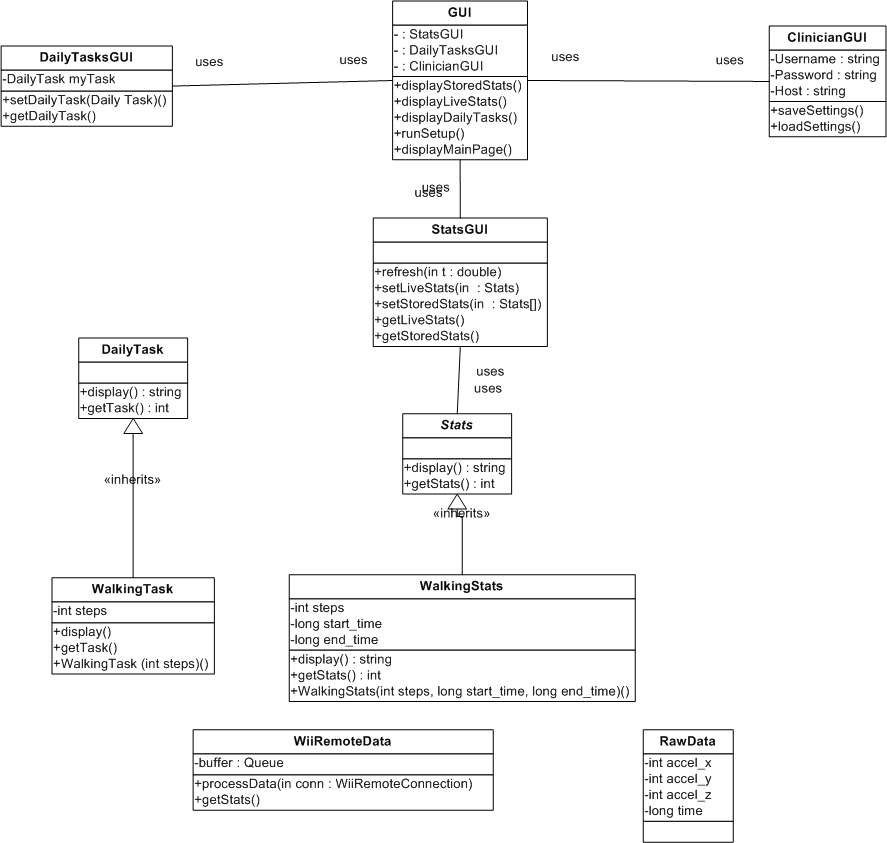
\includegraphics[width=6in,height=5.71in]{PDA_Patient_GUI.png}
\end{center}


\begin{longtable}[t]{|p{1.5in}|p{2in}|p{2.5in}|}

\hline
\textbf{Class} & \textbf{Method} & \textbf{Description} \\

\hline %Horizontal Bar accross table.

%This column spans multiple rows.
GUI

	%One row of the table.  '&' Is the column separator. '\\' Is the row terminator.
	& displayStoredStats() & This will bring up the GUI that will display the statistics from previous sessions. \\

	%Separate the two rows of the Server methods by a horizontal line. This is required.
	\cline{2-3}

	%Second row of the table.
  & displayLiveStats() & This will bring up the GUI that will display real time statistics that are currently being measured. \\
	\cline{2-3}

	%Second row of the table.
  & displayDailyTasks() & This will bring up the GUI that will display the daily tasks. \\
	\cline{2-3}

	%Second row of the table.
  & runSetup() & This will run the clinician setup and bring up the ClinicianGui so the clinician can enter the patients username, password and the host of the server's address. \\
  
  \cline{2-3}

	%Second row of the table.
  & displayMainPage() & This will display the main page that the user will see when they start the application. \\


\hline
Stats
		& display() & This is a pure virtual function that will display the PDA Statistics through an easy to read GUI. \\
		
		& getStats() & This is a pure virtual function that will retrieve the PDA Statistics. \\
\cline{2-3}

\hline
WalkingStats
		& display() & Virtual, derived function from the "Stats" abstract base. Displays the Walking Stats on the PDA through an easy to read GUI. \\
\cline{2-3}
		& getStats() & Retrieves the walking statistics to be displayed on the PDA. \\
\cline{2-3}
		& WalkingStats(int steps,$\newline$ long startTime, long endTime) & Constructor for the WalkingStats object that sets the object's attributes. \\
\cline{2-3}



\hline %Horizontal bar accross table.

%I got lazy and copied the second block. :-)
DailyTasksGui
      & setDailyTask(Daily Task) & This will set the Daily Task myTask with whatever is passed in to it. \\
\cline{2-3}
      & getDailyTask() & This will return an object of type Daily Task that has been stored in myTask. \\
\hline %Horizontal bar accross table.

WiiRemoteData
			& processData\newline(WiiRemoteConnection) & Periodically get the data from the provided WiiRemoteConnection and determine where the steps occur. \\
			\cline{2-3}
			& Stats getStats() & Return the next Stats object in the buffer. The Stats objects are created once enough raw data has been received. \\

\hline


ClinicianGUI

			& saveSettings() & Save the current settings to the configuration file. \\
			\cline{2-3}
			& loadSettings() & Load the settings saved in the configuration file if it exists. \\
\hline

DailyTask
			& string display() & Provides a human readable sentence indicating the task represented.\\
			\cline{2-3}
			
			& int *getTask() & Provides a pointer to either a single integer or an array of integer which can be used to represent the daily task. \\
			\cline{2-3}
			
\hline

WalkingTask
			& string display() & Provides a human readable sentence of the form: ``Walk xxx steps''. \\
			\cline{2-3}
			
			& int* getTask() & Provides a pointer to a single integer which represents the number of steps to walk that day. \\
			\cline{2-3}
			
			& WalkingTask(int steps) & Constructor which initializes the task to be walk the number of steps specified. \\
			
\hline

\end{longtable}

\subsubsection{PDA Alert Hierarchy}

\begin{center}
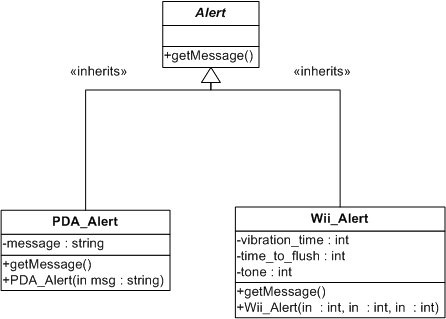
\includegraphics[width=3.72in,height=2.66in]{PDA_Alert_Hierarchy.png}
\end{center}


\begin{longtable}[t]{|p{1.5in}|p{2in}|p{2.5in}|}

\hline
\textbf{Class} & \textbf{Method} & \textbf{Description} \\
\hline

Alert
	& getMessage() & This will receive a message for an alert. \\
\hline %Horizontal bar accross table.

PDA\_Alert
	& getMessage() & This will receive a message for an alert to the PDA. \\
\cline{2-3}
      & PDA\_Alert(string) & This will alert the PDA with a certain message. \\
\hline %Horizontal bar accross table.

Wii\_Alert
	& getMessage() & This will receive a message for an alert to the Wii Remote. \\
\cline{2-3}
      & Wii\_Alert(int, int, int) & This will alert the Wii Remote with a certain vibration and flash time as well as tone. \\
\hline %Horizontal bar accross table.
\end{longtable}


\subsubsection{PDA-Server Connection}

\begin{center}
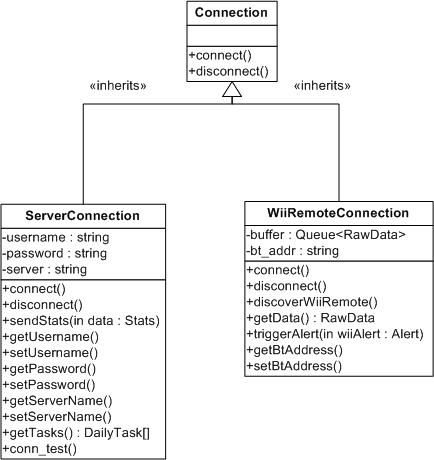
\includegraphics[width=3.62in,height=3.83in]{PDA_Server_Connection.png}
\end{center}


\begin{longtable}[t]{|p{1.5in}|p{2in}|p{2.5in}|}

\hline
\textbf{Class} & \textbf{Method} & \textbf{Description} \\
\hline %Horizontal Bar accross table.

%This column spans multiple rows.
Connection

	%One row of the table.  '&' Is the column separator. '\\' Is the row terminator.
	& connect() & This is a pure virtual function that will connect the PDA to the Server and Wii Remote respectively.  \\
	
	\cline{2-3}
	
	& disconnect() & This is a pure virtual function that will disconnect the PDA to the Server and Wii Remote respectively.  \\

	%Separate the two rows of the Server methods by a horizontal line. This is required.
	\cline{2-3}

\hline %Horizontal bar accross table.

ServerConnection
      & connect() & Virtual, derived function from the ``Connection'' abstract base. Connects the PDA to the server.  \\
      
      \cline{2-3}
      
      & disconnect() & Virtual, derived function from the ``Connection'' abstract base. Disconnects the PDA from the server.  \\
      
      \cline{2-3}
      
      & sendStats() & Sends PDA statistics to the server.  \\
      
      \cline{2-3}
      
      & getUsername() & Retrieves the username that the PDA will use to connect to the server.  \\
      
      \cline{2-3}
      
      & getPassword() & Retrieves the password that the PDA will use to connect to the server.  \\
      
      \cline{2-3}
      
      & setUsername() & Sets the username on the server that the PDA will connect to.  \\
      
      \cline{2-3}
      
      & setPassword() & Sets the password to the server that the PDA will connect to.  \\
      
      \cline{2-3}
      
      & getServerName() & Retrieves the server name that the PDA is connected to.  \\
      
      \cline{2-3}
      
      & setServerName() & Sets the name of the server that the PDA will connect to.  \\
      
      \cline{2-3}
      
      & getTasks() : DailyTask[] & Retrieves daily tasks for patient from the server as an array.  \\
      
      \cline{2-3}
      
      & conn\_test() & Runs a connection test to the server, returns status attempt to connect.  \\
      
\cline{2-3}

\hline 

WiiRemoteConnection
	  & connect() & Virtual, derived function from the ``Connection'' abstract base. Connects the PDA to the Wii Remote.  \\
      
      \cline{2-3}
      
      & disconnect() & Virtual, derived function from the ``Connection'' abstract base. Disconnects the PDA from the Wii Remote.  \\
      
      \cline{2-3}
      
      & discoverWiiRemote() & Function that looks for a Bluetooth Wii Remote that is specified by a Bluetooth address to be connected to the PDA.  \\
      
      \cline{2-3}
      
      & getData() : RawData & Retrieves data being sent by the Wii Remote and returns a RawData structure.  \\
      
      \cline{2-3}
      
      & triggerAlert(in wiiAlert:Alert) & This function takes an object of type Alert and will send the alert through to the PDA GUI.\\
      
      \cline{2-3}
      
      & getBtAddress() & Retrieves the Bluetooth address of the Wii Remote connected to the PDA.  \\
      
      \cline{2-3}
      
      & setBtAddress() & Sets the bluetooth address of the Wii Remote to be connected to the PDA.  \\
      
      \cline{2-3}


\hline
\end{longtable}

\subsection{Server Class Diagrams}

\subsubsection{Server WebUI}

\begin{center}
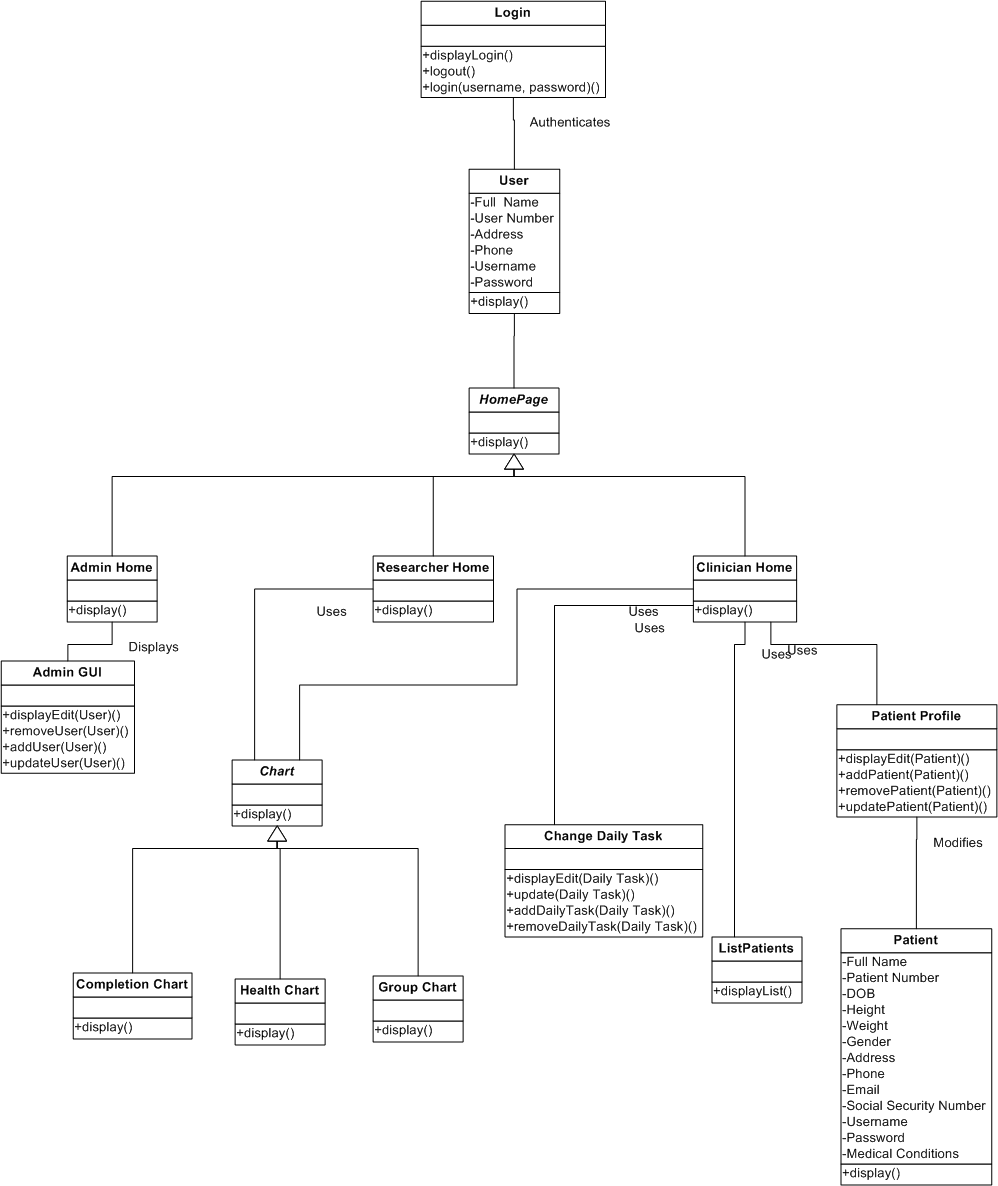
\includegraphics[width=6in,height=7.12in]{Server_Web_UI.png}
\end{center}

\newpage
\begin{longtable}[t]{|p{1.5in}|p{2in}|p{2.5in}|}

\hline
\textbf{Class} & \textbf{Method} & \textbf{Description} \\

\hline
AdminGUI
			& displayEdit(User) & Generates an editable form for modifying the fields associated with the provided user. If the User.Username field is blank this form will create a new user. Otherwise it will autofill the fields with the values provided by the User object. \\
			
			\cline{2-3}
			& removeUser(User) & Remove the user with User.Username from the database. \\
			\cline{2-3}
			& addUser(User) & Add a user to the database with the data provided by the User object. \\
			\cline{2-3}
			& updateUser(User) & Update the information in the database with the provided information for the user with username User.Username. \\
			
\hline

Login
      & displayLogin() & This will display the login page for all users. \\
\cline{2-3}
      & logout() & This will log the current user out. \\
\cline{2-3}
      & login(Username, Password) & This will take the populated fields for username and password, and return user type from the database if successful. \\
\hline %Horizontal bar accross table.

ListPatients
      & displayList() & This will give a list of all the clinician's patients on the interface. \\
\hline %Horizontal bar accross table.

PatientProfile
      & displayEdit(Patient) & This will take a Patient object as a parameter and display all the fields in editable form. \\
\cline{2-3}
      & addPatient(Patient) & This will take a Patient object as a parameter and add a new patient to the database. \\
\cline{2-3}
      & removePatient(Patient) & This will take a Patient object as a parameter and remove that patient from the database. \\
\cline{2-3}
      & updatePatient(Patient) & This will take a Patient object as a parameter and update an existing patient to the database. \\


\hline %Horizontal bar accross table.

%I got lazy and copied the second block. :-)
Chart
      & display() & Virtual function that will display the derived charts after getting the required data from the database. \\
\hline %Horizontal bar accross table.

%I got lazy and copied the second block. :-)
CompletionChart
      & display() & This function will display the patient completion charts by getting comparing patient statistics to the tasks that belong to them. \\
      %I wanted to end with "to"' but thats just bad grammar Im told
\hline %Horizontal bar accross table.

%I got lazy and copied the second block. :-)
GroupChart
      & display() & This function will gather data from a Clinician's or Researcher's group and graph it. \\
      
\hline %Horizontal bar accross table.

%I got lazy and copied the second block. :-)
HealthChart
      & display() & This function will get data that relates to the patients health and graph it. \\
      
      \hline
      
%This column spans multiple rows.
Homepage

	%One row of the table.  '&' Is the column separator. '\\' Is the row terminator.
	& display() & This is a pure virtual function that will display the respective homepages after a specific user (Clinician, Researcher, or Admin) logs into the Web UI.  \\

	%Separate the two rows of the Server methods by a horizontal line. This is required.
	\cline{2-3}

\hline %Horizontal bar accross table.

Admin Homepage
      & display() & Virtual, derived function from the ``Homepage'' abstract base. Displays the Admin's Homepage which allows the Admin to Add/Remove/Edit users of the Web UI.  \\
\cline{2-3}

\hline 

Researcher Homepage
		& display() & Virtual, derived function from the ``Homepage'' abstract base. Displays the Researcher's Homepage which gives the Researcher access to the Researcher Charts. \\
\cline{2-3}

\hline
Clinician Homepage
		& display() & Virtual, derived function from the ``Homepage'' abstract base. Displays the Clinician's Homepage which allows the Clinician to Manage Patients, Change Daily Tasks, and View Clinician Charts.\\
\cline{2-3}

\hline
Change Daily Task
		& displayEdit(Daily Task) & Shows the Daily Task specified as its argument in editable fields so that the Clinician can easily modify it. \\
\cline{2-3}
		& update(Daily Task) & Function that gets called to actually update the Daily Task after changes are made by the Clinician. \\
\cline{2-3}
		& addDailyTask(Daily Task) & Function that gets called when a new Daily Task is submitted by the Clinician. The function will take the Daily Task object and call the appropriate DAO to add it to the Database. \\
\cline{2-3}
		& removeDailyTask(Daily Task) & Function that gets called when a Daily Task is to be removed from a certain Patient's Profile. \\
		
\hline
\end{longtable}


\subsubsection{Server-PDA Connection}

\begin{center}
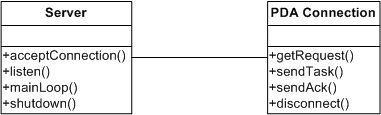
\includegraphics[width=3.18in,height=0.96in]{Server_PDA_Connection.png}
\end{center}


\begin{longtable}[t]{|p{1.5in}|p{2in}|p{2.5in}|}

\hline
\textbf{Class} & \textbf{Method} & \textbf{Description} \\
\hline %Horizontal Bar accross table.

%This column spans multiple rows.
Server

	& acceptConnection() & Accept a connection from PDA and create the PDAConnection object to associate with it. \\
	\cline{2-3}

	%Second row of the table.
  & listen() & Starts the listening socket. \\
	\cline{2-3}

	%One row of the table.  '&' Is the column separator. '\\' Is the row terminator.
	& mainLoop() & Called when initialized. This method opens a listening socket and waits for the PDA connections. \\

	%Separate the two rows of the Server methods by a horizontal line. This is required.
	\cline{2-3}

	& shutdown() & Close the listening socket and shutdown the server. \\
	
\hline %Horizontal bar accross table.

%I got lazy and only commented the first block. :-)
PDAConnection
      & getRequest() & Receive requests from the PDA and parse them into upload Stats or request of Daily Task messages. \\
\cline{2-3}
      & sendTask() & Send the daily task to the PDA. \\
\cline{2-3}
      & sendAck() & Send a ACK or NACK to the PDA to indicate whether the Stats were successfully received or not. \\
      \cline{2-3}
      & disconnect() & Break the connection with the associated PDA object. \\
\hline

\end{longtable}

\section{Unit Test Plan}

The convention for each method is to list the unique test identifier as the first paragraph. The unique test identifier is generated by taking the initials of the object subscript the initials of the method.

%%%%%%%%%%%%%%%%%%%%%%%%%%%%%%%%%%%%%%%%%%%%%%%%%%%%%%%%%%%%%%%%%%%%%%%%%%%%%%%%%%%%
%%%%%%%%%%%%%%%%%%%%%%%%%%%%%%%%%%%%%%%%%%%%%%%%%%%%%%%%%%%%%%%%%%%%%%%%%%%%%%%%%%%%
%%%%%%%%%%%%%%%%%%%%%%%%%%%%%%%%%%%%%%%%%%%%%%%%%%%%%%%%%%%%%%%%%%%%%%%%%%%%%%%%%%%%
%%%%%%%%%%%%%%%%%%%%%%%%%%%%%%%%%%%%%%%%%%%%%%%%%%%%%%%%%%%%%%%%%%%%%%%%%%%%%%%%%%%%
\subsection{PDA Patient GUI}

\subsubsection{GUI Object}

\paragraph{displayStoredStats()}

%The dollar signs have to be included because the underscore is a math symbol.
\subparagraph{GUI$_{dss}$}

\subparagraph{Risk Analysis}
This is a low risk system component due to the fact that it will just start up the StatsGUI function getStoredStats().

\subparagraph{Possible Defects}
If getStoredStats is not completed it will fail.

\subparagraph{Completion Criteria}
For this object to complete sucessfuly it will call the StatsGui function getStoredStats().



\paragraph{displayLiveStats()}

%The dollar signs have to be included because the underscore is a math symbol.
\subparagraph{GUI$_{dls}$}

\subparagraph{Risk Analysis}
This is a low risk system component due to the fact that it will just start up the StatsGUI function getLiveStats().

\subparagraph{Possible Defects}
If getLiveStats is not completed it will fail.

\subparagraph{Completion Criteria}
For this object to complete sucessfuly it will call the StatsGui function getLiveStats().

\paragraph{displayDailyTasks()}

%The dollar signs have to be included because the underscore is a math symbol.
\subparagraph{GUI$_{ddt}$}

\subparagraph{Risk Analysis}
This is a low risk system component due to the fact that it will just start up the DailyTasksGUI function getDailyTask().

\subparagraph{Possible Defects}
If getDailyTask is not completed it will fail.

\subparagraph{Completion Criteria}
For this object to complete sucessfuly it will call the DailyTasksGUI function getDailyTask().


\paragraph{runSetup()}

%The dollar signs have to be included because the underscore is a math symbol.
\subparagraph{GUI$_{rs}$}

\subparagraph{Risk Analysis}
This is a low risk system component due to the fact that it will just start up the ClinicianGUI.

\subparagraph{Possible Defects}
If the ClinicianGUI is not completed it will fail.


\subparagraph{Completion Criteria}
For this object to complete sucessfuly it will start the ClinicianGUI.


\paragraph{displayMainPage()}

%The dollar signs have to be included because the underscore is a math symbol.
\subparagraph{GUI$_{dmp}$}

\subparagraph{Risk Analysis}
This is a high risk system component due to it being the GUI from which all the navigation starts, and also returns to.

\subparagraph{Possible Defects}
The GUI not going to other GUI pages.

The GUI not displaying all options.

\subparagraph{Completion Criteria}
For this to be complete it must show all the options and travle to all the other GUI pages.

\subsubsection{ClinicianGUI}

\paragraph{saveSettings()}
\subparagraph{CGUI$_{ss}$}

\subparagraph{Risk Analysis}
This is a medium risk method. It is medium risk because it is responsible for file input and output with the configuration file. 

\subparagraph{Possible Defects}
\begin{enumerate}
\item A defect would be if the method wrote the wrong or incomplete settings to the configuration file.
\item Another defect would be if the settings were written in an incorrect format.
\item A third defect would be if the file was not closed properly preventing read/write access from other processes on the system.
\end{enumerate}

\subparagraph{Completion Criteria}
The function will be considered complete when it is capable of writing the settings to the configuration file and closing the file correctly. It must write the settings in the correct format so the settings can be loaded from the configuration file.

\paragraph{loadSettings()}
\subparagraph{CGUI$_{ls}$}

\subparagraph{Risk Analysis}
This is a medium risk to implement function because it requires file io. The function must retrieve the saved settings from the configuration file.

\subparagraph{Possible Defects}
\begin{enumerate}
\item The method incorrectly reads the format of the file and therefore the incorrect settings are loaded.
\item The file is incorrectly formatted to begin with and the function unknowingly loads the erroneous settings.
\item The file is not closed correctly once the settings are read into the system.
\end{enumerate}

\subparagraph{Completion Criteria}
The function will be considered complete when it correctly retrieves the settings from the configuration file and closes the file when finished.


\subsubsection{DailyTasksGui Object}

\paragraph{setDailyTask(Daily Task)}

%The dollar signs have to be included because the underscore is a math symbol.
\subparagraph{DTG$_{sdt}$}

\subparagraph{Risk Analysis}
This is a low risk system component because it just grabs a copy of daily task from the DailyTask object.

\subparagraph{Possible Defects}
If DailyTask has not been completed it may not return an object to DailyTasksGui.


\subparagraph{Completion Criteria}
This function needs DailyTask getTask() to return a DailyTask and it will store it in DailyTasksGUI.



\paragraph{getDailyTask()}

%The dollar signs have to be included because the underscore is a math symbol.
\subparagraph{DTG$_{gdt}$}

\subparagraph{Risk Analysis}
This is a meduim risk system component that will take the stored DailyTask and display it to the screen.

\subparagraph{Possible Defects}
If setDailyTask does not work then there will be no task to display.

\subparagraph{Completion Criteria}
The Daily Task needs to be displayed and it must let the user navigate back to the main page.


\subsubsection{WiiRemoteData Object}

\paragraph{processData(WiiRemoteConnection)}

%The dollar signs have to be included because the underscore is a math symbol.
\subparagraph{WRD$_{pd}$}

\subparagraph{Risk Analysis}
This is a high risk system component due to the constant need of reading in and processing new data. This could lead to memory leaks or delays in processing may crop up if the system is unable to process the data fast enough.

\subparagraph{Possible Defects}
\begin{enumerate}
\item The function is unable to handle the Wii Remote sampling rate and a backlog or RawData objects occurs. This would slow down system performance.
\item The function does not produce the correct Statistics objects when provided with predetermined data. 
\end{enumerate}
\subparagraph{Completion Criteria}
This method will be considered complete when it is capable of handling input data and producing the correct Stats objects for the WiiRemoteData internal buffer.  The data must be processed in real time and the amount of memory used by this component should not increase over time.

\paragraph{Stats getStats()}
\subparagraph{WRD$_{gs}$}

\subparagraph{Risk Analysis}
This is a low risk method because of it is a get method and only responsible for taking the next Stats object off the internal buffer.

\subparagraph{Possible Defects}
If the function does not remove the object it removes from the front of the queue it is considered a defect.

\subparagraph{Completion Criteria}
The method will be considered complete when it returns and removes the first Stats object from the internal queue.


\subsubsection{DailyTask}
Since this is an abstract data type it does not require a test plan.

\subsubsection{WalkingTask}

\paragraph{display()}
\subparagraph{WT$_{d}$}

\subparagraph{Risk Analysis}
This is a low risk function. The function is low risk, because it is responsible for taking the internal values of the object and creating a human readable sentence.

\subparagraph{Possible Defects}
If the function does not create a human readable sentence with the internal walking data then it is considered a defect.

\subparagraph{Completion Criteria}
The function will be complete when it creates a human readable sentence which can be used for display purposes that represents the internal data of the object.

\paragraph{getStats()}
\subparagraph{WT$_{gs}$}

\subparagraph{Risk Analysis}
This is a low risk method. It is considered low risk because it is a get method and involves no serious data processing.

\subparagraph{Possible Defects}
If the method returns a pointer to an array of integers located on the stack instead of on the heap it will be considered defective.

\subparagraph{Completion Criteria}
The method will be considered complete when it returns a pointer to a heap allocated array of integers representing the internal data of the object.

\paragraph{WalkingTask(int steps)}
\subparagraph{WT$_{wt}$}

\subparagraph{Risk Analysis}
This is a low risk method, because it is responsible for setting the internal data member of the object. There is no data processing or allocation of resources involved.

\subparagraph{Possible Defects}
If the internal data member is not set to the provided value the method is defective.

\subparagraph{Completion Criteria}
If the method takes an input value and sets the internal data member of the object to the input then the method will be considered completed.

\subsubsection{Stats Object}

\paragraph{display()}

%The dollar signs have to be included because the underscore is a math symbol.
\subparagraph{ST$_{d}$}

\subparagraph{Risk Analysis}
This is a low risk system component due to the fact that it will just call the display function from a specific Stats object.

\subparagraph{Possible Defects}
The display function is not called.

\subparagraph{Completion Criteria}
The stats are displayed.

\paragraph{getStats()}

%The dollar signs have to be included because the underscore is a math symbol.
\subparagraph{ST$_{gs}$}

\subparagraph{Risk Analysis}
This is a low risk system component due to the fact that it will just call the getStats() function from a specific Stats object.

\subparagraph{Possible Defects}
The statistics are not retrieved.

\subparagraph{Completion Criteria}
The statistics are retrieved.


\subsubsection{WalkingStats Object}

\paragraph{display()}

%The dollar signs have to be included because the underscore is a math symbol.
\subparagraph{WST$_{d}$}

\subparagraph{Risk Analysis}
This is a low risk system component due to the fact that it will just display the task attributes.

\subparagraph{Possible Defects}
The Walking Task is incorrectly displayed.

\subparagraph{Completion Criteria}
The Walking Task is displayed correctly.

\paragraph{getStats()}

%The dollar signs have to be included because the underscore is a math symbol.
\subparagraph{WST$_{gs}$}

\subparagraph{Risk Analysis}
This is a low risk system component due to the fact that it will just retrieve the attributes stored in the object.

\subparagraph{Possible Defects}
The attributes are not returned.

\subparagraph{Completion Criteria}
The task attributes are retrieved.

\paragraph{WalkingTask(int steps, long start\_time, long end\_time)}

%The dollar signs have to be included because the underscore is a math symbol.
\subparagraph{WST$_{wt}$}

\subparagraph{Risk Analysis}
This is a low risk system component due to the fact that it will just set the objects attributes.

\subparagraph{Possible Defects}
The attributes are not set correctly.

\subparagraph{Completion Criteria}
The object's attributes are set correctly.

%%%%%%%%%%%%%%%%%%%%%%%%%%%%%%%%%%%%%%%%%%%%%%%%%%%%%%%%%%%%%%%%%%%%%%%%%%%%%%%%%%%%
%%%%%%%%%%%%%%%%%%%%%%%%%%%%%%%%%%%%%%%%%%%%%%%%%%%%%%%%%%%%%%%%%%%%%%%%%%%%%%%%%%%%
%%%%%%%%%%%%%%%%%%%%%%%%%%%%%%%%%%%%%%%%%%%%%%%%%%%%%%%%%%%%%%%%%%%%%%%%%%%%%%%%%%%%
%%%%%%%%%%%%%%%%%%%%%%%%%%%%%%%%%%%%%%%%%%%%%%%%%%%%%%%%%%%%%%%%%%%%%%%%%%%%%%%%%%%%
\subsection{PDA Alert Hierarchy}

\subsubsection{Alert Object}

\paragraph{getMessage()}

%The dollar signs have to be included because the underscore is a math symbol.
\subparagraph{Alert$_{gm}$}

\subparagraph{Risk Analysis}
This has a low risk factor since it just receives a message for an alert.

\subparagraph{Possible Defects}
No alert will occur without a message being received.

\subparagraph{Completion Criteria}
For the completion to be successful it will receive a message for the alert to be called.


\subsubsection{PDAAlert Object}

\paragraph{getMessage()}

%The dollar signs have to be included because the underscore is a math symbol.
\subparagraph{PDAAlert$_{gm}$}

\subparagraph{Risk Analysis}
This has a low risk factor since it just receives a message for an alert for the PDA.

\subparagraph{Possible Defects}
No alert will occur without a message being received for the PDA.

\subparagraph{Completion Criteria}
For the completion to be successful it will receive a message for the alert to be called on the PDA.


\paragraph{PDAAlert(string)}

%The dollar signs have to be included because the underscore is a math symbol.
\subparagraph{PDAAlert$_{pa}$}

\subparagraph{Risk Analysis}
This has a low risk factor since it just alerts the PDA with a message.

\subparagraph{Possible Defects}
No alert will occur if there isn't a message for the parameter.

\subparagraph{Completion Criteria}
For the completion to be successful it will display an alert on the PDA with a certain message.


\subsubsection{WiiAlert Object}

\paragraph{getMessage()}

%The dollar signs have to be included because the underscore is a math symbol.
\subparagraph{WiiAlert$_{gm}$}

\subparagraph{Risk Analysis}
This has a low risk factor since it just receives a message for an alert for the Wii Remote.

\subparagraph{Possible Defects}
No alert will occur without a message being received for the Wii Remote.

\subparagraph{Completion Criteria}
For the completion to be successful it will receive a message for the alert on the Wii Remote.


\paragraph{WiiAlert(int,int,int)}

%The dollar signs have to be included because the underscore is a math symbol.
\subparagraph{WiiAlert$_{wa}$}

\subparagraph{Risk Analysis}
This has a medium risk factor because it alerts the Wii Remote with vibrations and flashes for notification.

\subparagraph{Possible Defects}
No alert will occur and the client will not be notified for any progress.

\subparagraph{Completion Criteria}
For the completion to be successful it will alert the Wii Remote with vibration and flash times.




%%%%%%%%%%%%%%%%%%%%%%%%%%%%%%%%%%%%%%%%%%%%%%%%%%%%%%%%%%%%%%%%%%%%%%%%%%%%%%%%%%%%
%%%%%%%%%%%%%%%%%%%%%%%%%%%%%%%%%%%%%%%%%%%%%%%%%%%%%%%%%%%%%%%%%%%%%%%%%%%%%%%%%%%%
%%%%%%%%%%%%%%%%%%%%%%%%%%%%%%%%%%%%%%%%%%%%%%%%%%%%%%%%%%%%%%%%%%%%%%%%%%%%%%%%%%%%
%%%%%%%%%%%%%%%%%%%%%%%%%%%%%%%%%%%%%%%%%%%%%%%%%%%%%%%%%%%%%%%%%%%%%%%%%%%%%%%%%%%%
\subsection{PDA-Server Connection}

\subsubsection{Connection}

\paragraph{connect()}

%The dollar signs have to be included because the underscore is a math symbol.
\subparagraph{Connection$_{con}$}

\subparagraph{Risk Analysis}
This is a low risk system component due to the fact that it will just call the appropriate connect() function in either the WiiRemoteConnection or ServerConnection object.

\subparagraph{Possible Defects}
If connect is not completed the system may not have all of its compnents connected and will fail.

\subparagraph{Completion Criteria}
For this object to complete sucessfuly it will call the appropriate connect() function in either the WiiRemoteConnection or ServerConnection object.



\paragraph{disconnect()}

%The dollar signs have to be included because the underscore is a math symbol.
\subparagraph{Connection$_{dis}$}

\subparagraph{Risk Analysis}
This is a low risk system component due to the fact that it will just call the appropriate disconnect() function in either the WiiRemoteConnection or ServerConnection object.

\subparagraph{Possible Defects}
If disconnect is not completed the system may have components still connected when they should not be.

\subparagraph{Completion Criteria}
For this object to complete sucessfuly it will call the appropriate disconnect() function in either the WiiRemoteConnection or ServerConnection object.



\subsubsection{ServerConnection Object}

\paragraph{connect()}

%The dollar signs have to be included because the underscore is a math symbol.
\subparagraph{SC$_{conn}$}

\subparagraph{Risk Analysis}
This is a high risk system component because it is the method for which the PDA connects to the Server.

\subparagraph{Possible Defects}
If connect() has not been completed the data flow between the PDA and server cannot be completed or started.

\subparagraph{Completion Criteria}
The PDA connects to the server.


\paragraph{disconnect()}

%The dollar signs have to be included because the underscore is a math symbol.
\subparagraph{SC$_{dis}$}

\subparagraph{Risk Analysis}
This is a low risk system component that will disconnect the PDA from the server.

\subparagraph{Possible Defects}
If PDA does not disconnect, will not impact system.

\subparagraph{Completion Criteria}
The PDA is disconnected from the server.

\paragraph{sendStats()}

%The dollar signs have to be included because the underscore is a math symbol.
\subparagraph{SC$_{ss}$}

\subparagraph{Risk Analysis}
This is a meduim risk system component that will send the stored stats on the PDA to the server.

\subparagraph{Possible Defects}
If sendStats() does not work, the server will not be able to collect patient data.

\subparagraph{Completion Criteria}
The Server needs to receive stats sent by the PDA.

\paragraph{getUsername()}

%The dollar signs have to be included because the underscore is a math symbol.
\subparagraph{SC$_{gun}$}

\subparagraph{Risk Analysis}
This is a medium risk system component that will retrieve the username the PDA needs to connect to the server.

\subparagraph{Possible Defects}
If getUsername does not work the PDA will unable to use the correct credentials to connect to the server.

\subparagraph{Completion Criteria}
The PDA retrieves the username for the server.

\paragraph{getPassword()}

%The dollar signs have to be included because the underscore is a math symbol.
\subparagraph{SC$_{gpw}$}

\subparagraph{Risk Analysis}
This is a meduim risk system component that will retrieve the password the PDA needs to connect to the server.

\subparagraph{Possible Defects}
If getPassword does not work the PDA will unable to use the correct credentials to connect to the server.

\subparagraph{Completion Criteria}
The PDA retrieves the password for the server.

\paragraph{setUsername()}

%The dollar signs have to be included because the underscore is a math symbol.
\subparagraph{SC$_{sun}$}

\subparagraph{Risk Analysis}
This is a meduim risk system component that will set the username that the PDA uses to connect to the server.

\subparagraph{Possible Defects}
If setUsername() does not work, the username required to connect to the server may not be updated.

\subparagraph{Completion Criteria}
The username stored on the PDA to connect to the server is changed.

\paragraph{setPassword()}

%The dollar signs have to be included because the underscore is a math symbol.
\subparagraph{SC$_{spw}$}

\subparagraph{Risk Analysis}
This is a meduim risk system component that will set the password that the PDA uses to connect to the server.

\subparagraph{Possible Defects}
If setPassword() does not work, the username required to connect to the server may not be updated.

\subparagraph{Completion Criteria}
The password stored on the PDA to connect to the server is changed.

\paragraph{getServerName()}

%The dollar signs have to be included because the underscore is a math symbol.
\subparagraph{SC$_{gsn}$}

\subparagraph{Risk Analysis}
This is a medium risk system component that will retrieve the Server Name the PDA needs to connect to the server.

\subparagraph{Possible Defects}
If getServerName does not work the PDA will unable to use the correct credentials to connect to the server.

\subparagraph{Completion Criteria}
The PDA retrieves the Server Name for the server.

\paragraph{setServerName()}

%The dollar signs have to be included because the underscore is a math symbol.
\subparagraph{SC$_{ssn}$}

\subparagraph{Risk Analysis}
This is a meduim risk system component that will set the Server Name that the PDA uses to connect to the server.

\subparagraph{Possible Defects}
If setServerName() does not work, the Server Name required to connect to the server may not be updated.

\subparagraph{Completion Criteria}
The Server Name stored on the PDA to connect to the server is changed.

\paragraph{getTasks()}

%The dollar signs have to be included because the underscore is a math symbol.
\subparagraph{SC$_{gt}$}

\subparagraph{Risk Analysis}
This is a high risk system component that will retireve an array of daily tasks from the server.

\subparagraph{Possible Defects}
If getTasks does not work then there will be no tasks on the PDA.

\subparagraph{Completion Criteria}
The PDA is able to display new daily tasks retrieved from the server.

\paragraph{conn\_test()}

%The dollar signs have to be included because the underscore is a math symbol.
\subparagraph{SC$_{connt}$}

\subparagraph{Risk Analysis}
This is a meduim risk system component that will test the connection to the Server.

\subparagraph{Possible Defects}
If conn\_test() fails, then there will be no way to tell if the connection to the server is valid.

\subparagraph{Completion Criteria}
The conn\_test() function returns the correct status of the Server to PDA connection.

\subsubsection{WiiRemoteConnection Object}

\paragraph{connect()}

%The dollar signs have to be included because the underscore is a math symbol.
\subparagraph{WRC$_{conn}$}

\subparagraph{Risk Analysis}
This is a high risk system component because it is the method for which the PDA connects to the Wii Remote.

\subparagraph{Possible Defects}
If connect() has not been completed the data flow between the PDA and Wii Remote cannot be completed or started.

\subparagraph{Completion Criteria}
The PDA connects to the Wii Remote.

\paragraph{disconnect()}

%The dollar signs have to be included because the underscore is a math symbol.
\subparagraph{WRC$_{dis}$}

\subparagraph{Risk Analysis}
This is a low risk system component that will disconnect the PDA from the Wii Remote.

\subparagraph{Possible Defects}
If PDA does not disconnect, will not impact system.

\subparagraph{Completion Criteria}
The PDA is disconnected from the Wii Remote.

\paragraph{discoverWiiRemote()}

%The dollar signs have to be included because the underscore is a math symbol.
\subparagraph{WRC$_{dwr}$}

\subparagraph{Risk Analysis}
This is a high risk system component as the PDA needs to discover the Wii Remote to connect to it.

\subparagraph{Possible Defects}
The PDA is incapable of discovering Blue tooth Wii Remote
.
\subparagraph{Completion Criteria}
PDA recognizes Wii Remote device.

\paragraph{getData()}

%The dollar signs have to be included because the underscore is a math symbol.
\subparagraph{WRC$_{gd}$}

\subparagraph{Risk Analysis}
This is a high risk system component as processing Wii Remote data is the main function of the system.

\subparagraph{Possible Defects}
Wii Remote data is not returned.

\subparagraph{Completion Criteria}
Wii Remote data is received on the PDA and able to be processed.

\paragraph{triggerAlert(Alert)}

%The dollar signs have to be included because the underscore is a math symbol.
\subparagraph{WRC$_{tra}$}

\subparagraph{Risk Analysis}
This is a low risk system component as alerts are not necessary for core system functionailty of processing data.

\subparagraph{Possible Defects}
Alert is not triggered when an event that should trigger one occurs.
\subparagraph{Completion Criteria}
PDA alert appears to patient when appropriate event occurs.

\paragraph{getBtAddress()}

%The dollar signs have to be included because the underscore is a math symbol.
\subparagraph{WRC$_{gbta}$}

\subparagraph{Risk Analysis}
This is a medium risk system component since retrieving the Bluetooth address of the Wii Remote is necessary for proper connection.

\subparagraph{Possible Defects}
PDA unable to determine address of Wii Remote.
\subparagraph{Completion Criteria}
PDA recognizes bluetooth address of Wii Remote.

\paragraph{setBtAddress()}

%The dollar signs have to be included because the underscore is a math symbol.
\subparagraph{WRC$_{sbta}$}

\subparagraph{Risk Analysis}
This is a medium risk system component since the result of setting the bluetooth address impacts the PDA's ability to connect to the Wii Remote.

\subparagraph{Possible Defects}
PDA does not overwrite bluetooth address stored on PDA, unable to pair device.
\subparagraph{Completion Criteria}
Bluetooth address for Wii Remote updated on PDA.


%%%%%%%%%%%%%%%%%%%%%%%%%%%%%%%%%%%%%%%%%%%%%%%%%%%%%%%%%%%%%%%%%%%%%%%%%%%%%%%%%%%%
%%%%%%%%%%%%%%%%%%%%%%%%%%%%%%%%%%%%%%%%%%%%%%%%%%%%%%%%%%%%%%%%%%%%%%%%%%%%%%%%%%%%
%%%%%%%%%%%%%%%%%%%%%%%%%%%%%%%%%%%%%%%%%%%%%%%%%%%%%%%%%%%%%%%%%%%%%%%%%%%%%%%%%%%%
%%%%%%%%%%%%%%%%%%%%%%%%%%%%%%%%%%%%%%%%%%%%%%%%%%%%%%%%%%%%%%%%%%%%%%%%%%%%%%%%%%%%
\subsection{Server WebUI}

\paragraph{ListPatients()}

%The dollar signs have to be included because the underscore is a math symbol.
\subparagraph{GUI$_{lp}$}

\subparagraph{Risk Analysis}
This has a medium risk factor because it displays a list of all a client's patients.

\subparagraph{Possible Defects}
No list of patients will be displayed and further analysis can not be implemented.

\subparagraph{Completion Criteria}
For the completion to be successful it will display a list of all a client's patients on the UI.

\subsubsection{Login Object}

\paragraph{displayLogin()}

%The dollar signs have to be included because the underscore is a math symbol.
\subparagraph{Login$_{dl}$}

\subparagraph{Risk Analysis}
This has a medium risk factor since it just displays the login page.

\subparagraph{Possible Defects}
The login page will not display and nobody can login to their account.

\subparagraph{Completion Criteria}
For the completion to be successful it display the login page for all users.

\paragraph{logout()}

%The dollar signs have to be included because the underscore is a math symbol.
\subparagraph{Login$_{lo}$}

\subparagraph{Risk Analysis}
This has a low risk factor since it just signs a user out of his/her account.

\subparagraph{Possible Defects}
The user will not be able to logout of their account.

\subparagraph{Completion Criteria}
For the completion to be successful it will end a current user's session.

\paragraph{login(Username,Password)}

%The dollar signs have to be included because the underscore is a math symbol.
\subparagraph{Login$_{li}$}

\subparagraph{Risk Analysis}
This has a medium risk factor because it instiantiates a session for a user on the UI.

\subparagraph{Possible Defects}
No user will be able to log into the system.

\subparagraph{Completion Criteria}
For the completion to be successful a user will be able to log into the system and return user type from the database.


\subsubsection{PatientProfile Object}

\paragraph{displayEdit(Patient)}

%The dollar signs have to be included because the underscore is a math symbol.
\subparagraph{PP$_{de}$}

\subparagraph{Risk Analysis}
This has a medium risk factor because it displays edit for patient profiles.

\subparagraph{Possible Defects}
The user is not able to see patients' credentials in editable form.

\subparagraph{Completion Criteria}
For the completion to be successful it populates the UI with the patient profile in editable form.

\paragraph{addPatient(Patient)}

%The dollar signs have to be included because the underscore is a math symbol.
\subparagraph{PP$_{ap}$}

\subparagraph{Risk Analysis}
This has a medium risk factor because it allows addition of patients.

\subparagraph{Possible Defects}
Patients can not be added into the database.

\subparagraph{Completion Criteria}
For the completion to be successful a patient is securely added into the back-end.

\paragraph{removePatient(Patient)}

%The dollar signs have to be included because the underscore is a math symbol.
\subparagraph{PP$_{rp}$}

\subparagraph{Risk Analysis}
This has a low risk factor because it just deletes unused patients from the database.

\subparagraph{Possible Defects}
Patients can not be deleted once added to the database.

\subparagraph{Completion Criteria}
For the completion to be successful it removes a patient completely from the back-end.

\paragraph{updatePatient(Patient)}

%The dollar signs have to be included because the underscore is a math symbol.
\subparagraph{PP$_{de}$}

\subparagraph{Risk Analysis}
This has a medium risk factor because it allows edit for patient profiles.

\subparagraph{Possible Defects}
Patients can not be edited once added to the database.

\subparagraph{Completion Criteria}
For the completion to be successful a patient can be modified after being added to the back-end.


\subsubsection{AdminGUI}

\paragraph{displayEdit(User)}

\subparagraph{AGUI$_{de}$}

\subparagraph{Risk Analysis}
This is a low risk method because its primary purpose is to generate html code to display to the user. The html code should produce the edit user interface for the Admin user.

\subparagraph{Possible Defects}
\begin{enumerate}
\item If the page is not displayed as the GUI mockup indicates.
\item The page does not contain the initial values of all the fields when editing an existing user.
\end{enumerate}

\subparagraph{Completion Criteria}
The function will be considered complete when the output is a syntactically correct html string which when shown in a browser displays the edit user gui as drawn in the GUI mockups.


\paragraph{removeUser(User)}
\subparagraph{AGUI$_{ru}$}

\subparagraph{Risk Analysis}
This is a medium risk function. The function is medium risk because it must remove a user from the database.

\subparagraph{Possible Defects}
\begin{enumerate}
\item The user is not removed from the database.
\item The wrong user is removed from the database, or unnecessary user data is removed from the database.
\end{enumerate}

\subparagraph{Completion Criteria}
The function will be considered complete when it removes only the user specified from the database.


\paragraph{addUser(User)}
\subparagraph{AGUI$_{au}$}

\subparagraph{Risk Analysis}
This is a low risk function because it is inserting a record into the database.

\subparagraph{Possible Defects}
\begin{enumerate}
\item The wrong user object is created.
\item The user object is created when a user of that username already exists.
\end{enumerate}

\subparagraph{Completion Criteria}
The function will be considered complete when a new user record is created in the database for a new unique User object that has been specified. If the username is already in use the function should return an error.


\paragraph{updateUser(User)}
\subparagraph{AGUI$_{uu}$}

\subparagraph{Risk Analysis}
This is a medium risk function due to the need to update a record in the database.

\subparagraph{Possible Defects}
\begin{enumerate}
\item The wrong record is updated, or no record is updated at all.
\item If no record is updated and an error message is not returned.
\end{enumerate}

\subparagraph{Completion Criteria}
The function will be considered complete when the User object is successfully propagated onto the database. In other words, the correct record is updated with the correct values. If an error occurs, the function should return the appropriate error code.


\subsubsection{Chart Object}

\paragraph{display()}

%The dollar signs have to be included because the underscore is a math symbol.
\subparagraph{C$_{d}$}

\subparagraph{Risk Analysis}
This is a low risk system component due to the the fact that nothing relies on the charts to complete.

\subparagraph{Possible Defects}
Since this is a virtual function there should be no defects.
\subparagraph{Completion Criteria}
Since this is a virtual function there should be no test for completion.





\subsubsection{CompletonChart Object}

\paragraph{display()}

%The dollar signs have to be included because the underscore is a math symbol.
\subparagraph{CC$_{d}$}

\subparagraph{Risk Analysis}
This is a low risk system component due to the the fact that nothing relies on the charts to complete.

\subparagraph{Possible Defects}
The chart might not display or might not display the correct information.

\subparagraph{Completion Criteria}
The chart displays the correctly.

\subsubsection{GroupChart Object}

\paragraph{display()}

%The dollar signs have to be included because the underscore is a math symbol.
\subparagraph{GC$_{d}$}

\subparagraph{Risk Analysis}
This is a low risk system component due to the the fact that nothing relies on the charts to complete.

\subparagraph{Possible Defects}
The chart might not display or might not display the correct information.

\subparagraph{Completion Criteria}
The chart displays the correctly.





\subsubsection{HealthChart Object}

\paragraph{display()}

%The dollar signs have to be included because the underscore is a math symbol.
\subparagraph{HC$_{d}$}

\subparagraph{Risk Analysis}
This is a low risk system component due to the the fact that nothing relies on the charts to complete.

\subparagraph{Possible Defects}
The chart might not display or might not display the correct information.

\subparagraph{Completion Criteria}
The chart displays the correctly.


\subsubsection{Admin HomePage}

\paragraph{display()}

%The dollar signs have to be included because the underscore is a math symbol.
\subparagraph{AH$_{d}$}

\subparagraph{Risk Analysis}
This is a medium risk system component. Researchers and Clinicians can always be added to the database manually, but a GUI is desirable.

\subparagraph{Possible Defects}
The wrong homepage may be displayed. For example, a Clinician logs in and is brought to the Admin Homepage. 

\subparagraph{Completion Criteria}
The Admin logs into the Web UI through the login screen. The Admin is presented with a GUI representing their homepage. From here,
the Admin can add/remove/edit Clinicians and Researchers.

\subsubsection{Clinician HomePage}

\paragraph{display()}

%The dollar signs have to be included because the underscore is a math symbol.
\subparagraph{CH$_{d}$}

\subparagraph{Risk Analysis}
This is a high risk component. This module must be implemented correctly in order for the Clinician to inteface with the application and access core system functionality.

\subparagraph{Possible Defects}
\begin{enumerate}
\item The wrong homepage may be displayed
\item The homepage may not include all required functionality: Patient List, Add Patient, Modify Daily Tasks and Logout
\end{enumerate}


\subparagraph{Completion Criteria}
The Clinician logs into the Web UI through the login screen. The Clinician is presented with a GUI representing their homepage. The Clinician is presented with the toolbar on the left-hand side
that allows the Clinician to access their Patient List, Add/Edit Patients (which includes the Modification of the Daily Tasks), and Logout.


\subsubsection{Researcher HomePage}

\paragraph{display()}

%The dollar signs have to be included because the underscore is a math symbol.
\subparagraph{RH$_{d}$}

\subparagraph{Risk Analysis}
This is a medium risk component. This module must be implemented correctly in order for the Researcher to inteface with the application to access Researcher Charts.

\subparagraph{Possible Defects}
\begin{enumerate}
\item The wrong homepage may be displayed
\item The homepage may not include all required functionality: View Group Patient Charts, Completion Charts, and Health Charts.
\end{enumerate}


\subparagraph{Completion Criteria}
The Researcher logs into the Web UI through the login screen. The Researcher is presented with a GUI representing their homepage. The Researcher is presented with the toolbar on the left-hand side
that allows the Researcher to access all of the Researcher Charts (Completion, Health, and Group).

\subsubsection{Change Daily Task}

\paragraph{displayEdit(Daily Task)}

%The dollar signs have to be included because the underscore is a math symbol.
\subparagraph{CDT$_{de}$}

\subparagraph{Risk Analysis}
This is a high risk component. This module must be implemented correctly in order for the Clinician assign Daily Tasks to a Patient.

\subparagraph{Possible Defects}
The wrong Daily Task may be displayed.


\subparagraph{Completion Criteria}
This method will be considered complete when the Clinician is able to edit a Daily Task from the Patient Profile screen. The Edit Daily Task screen will allow 
the Clinician to edit the number of steps the Patient is supposed to walk. 

\paragraph{update(Daily Task)}

%The dollar signs have to be included because the underscore is a math symbol.
\subparagraph{CDT$_{u}$}

\subparagraph{Risk Analysis}
This is a high risk component. This module must be implemented correctly in order for the Clinician assign Daily Tasks to a Patient.

\subparagraph{Possible Defects}
\begin{enumerate}
\item The wrong Daily Task gets updated.
\item Multiple Daily Tasks get updated. 
\item The correct Daily Task gets updated with the wrong value(s). 
\end{enumerate}

\subparagraph{Completion Criteria}
This method will be considered complete when the the correct Daily Task is actually updated in the database after the Clinician modifies it in the GUI.

\paragraph{addDailyTask(Daily Task)}

%The dollar signs have to be included because the underscore is a math symbol.
\subparagraph{CDT$_{adt}$}

\subparagraph{Risk Analysis}
This is a high risk component. This module must be implemented correctly in order for the Clinician assign Daily Tasks to a Patient.

\subparagraph{Possible Defects}
The wrong Daily Task gets added

\subparagraph{Completion Criteria}
This method will be considered complete when the the correct Daily Task is actually added into the database after the Clinician adds it via the Web UI.

\paragraph{removeDailyTask(Daily Task)}

%The dollar signs have to be included because the underscore is a math symbol.
\subparagraph{CDT$_{rdt}$}

\subparagraph{Risk Analysis}
This is a high risk component. This module must be implemented correctly in order for the Clinician remove Daily Tasks to a Patient.

\subparagraph{Possible Defects}
\begin{enumerate}
\item The wrong Daily Task gets removed from the database.
\item Multiple Daily Tasks get removed from the database. 
\end{enumerate}

\subparagraph{Completion Criteria}
This method will be considered complete when the the correct Daily Task is actually removed into the database after the Clinician removes it via the Web UI.


%%%%%%%%%%%%%%%%%%%%%%%%%%%%%%%%%%%%%%%%%%%%%%%%%%%%%%%%%%%%%%%%%%%%%%%%%%%%%%%%%%%%
%%%%%%%%%%%%%%%%%%%%%%%%%%%%%%%%%%%%%%%%%%%%%%%%%%%%%%%%%%%%%%%%%%%%%%%%%%%%%%%%%%%%
%%%%%%%%%%%%%%%%%%%%%%%%%%%%%%%%%%%%%%%%%%%%%%%%%%%%%%%%%%%%%%%%%%%%%%%%%%%%%%%%%%%%
%%%%%%%%%%%%%%%%%%%%%%%%%%%%%%%%%%%%%%%%%%%%%%%%%%%%%%%%%%%%%%%%%%%%%%%%%%%%%%%%%%%%
\subsection{Server-PDA Connection}

\subsubsection{Server}
\paragraph{acceptConnection()}
\subparagraph{S$_{ac}$}

\subparagraph{Risk Analysis}
This is a low risk component as an accept connection routine is common to many servers already in existence. Therefore the design of this function is known.

\subparagraph{Possible Defects}
\begin{enumerate}
\item A possible defect is if the server did not accept the connection and allocate the resources required by the new connection. This allocation must occur in order to proceed.
\item Another defect would be if the server refused to accept connections.
\end{enumerate}

\subparagraph{Completion Criteria}
This item will be considered complete when it successfully accepts an incoming connection from a PDA and instantiates the correct objects to handle the remainder of the connection processing.  It must also successfully pass the accepted client Socket connection off to the newly instantiated objects.

\paragraph{listen()}
\subparagraph{S$_{l}$}

\subparagraph{Risk Analysis}
This is another low risk function due to its common nature among servers. As long as the standard server model is followed there should be minimal risk.

\subparagraph{Possible Defects}
One defect would be if the server did not open a secure port of listening. 

\subparagraph{Completion Criteria}
This method will be considered complete when a secure port on the server machine has been opened and the necessary parameters have been passed to the acceptConnection function or saved in the object.

\paragraph{mainLoop()}
\subparagraph{S$_{ml}$}

\subparagraph{Risk Analysis}
This is another low risk function.  Since it is only responsible for controlling the server and ensuring user commands are executed it, there are few opportunities for issues to arise.

\subparagraph{Possible Defects}
\begin{enumerate}
\item A possible defect is if the function is unable to parse user input correctly.
\item Another defect would be if the input prompt freezes when attempting to perform an operation on the server.
\item The loop must not exist unless the user specifically requests the loop to terminate.
\end{enumerate}

\subparagraph{Completion Criteria}
The function will be considered complete when the user is able to enter control commands and the commands are correctly distributed to the appropriate function within the server. 

\subsubsection{PDAConnections}
\paragraph{getRequest()}
\subparagraph{PDAC$_{gr}$}

\subparagraph{Risk Analysis}
This is a medium risk function as it is responsible for receiving all requests from the PDA and parsing them appropriately.  This is reliant upon the successfully completion of a message protocol which will be used by both the PDA application and this function.

\subparagraph{Possible Defects}
\begin{enumerate}
\item Defects include losing complete requests which follow an incomplete request.
\item Also allocating resources for an incomplete or incorrect request is considered a defect.
\item A third defect is if the function does not exist gracefully when the socket layer connection is terminated.
\end{enumerate}

\subparagraph{Completion Criteria}
The function will be considered complete when it successfully receives a request from the PDA and successfully passes it to the appropriate request handler. If an erroneous request is received it should be ignore and the function should continue.  When the socket connection is terminated the function should exit gracefully.

\paragraph{sendTask()}
\subparagraph{PDAC$_{st}$}

\subparagraph{Risk Analysis}
This is a medium risk method to implement. It must be able to respond to a send task request from the PDA using the appropriate message format. It must be able to successfully translate from the Stats object to a message.

\subparagraph{Possible Defects}
A possible defect would be if the object was incorrectly translated to a message.

\subparagraph{Completion Criteria}
It will be complete when it is capable of sending a Stats object over the PDA socket connection using the appropriate message format.


\paragraph{sendAck(boolean ack)}

\subparagraph{PDAC$_{sa}$}

\subparagraph{Risk Analysis}
This is a low risk method, because it must respond to the PDA with a ACK message or a NACK message.

\subparagraph{Possible Defects}
If the messages do not follow the prescribed protocol, this is considered a defect.

\subparagraph{Completion Criteria}
The task will be considered complete when the functions ends a properly formated ACK or NACK message depending upon the input parameter. An input of true should send an ACK message, while an input of false should send a NACK message.

\paragraph{disconnect()}
\subparagraph{PDAC$_{d}$}

\subparagraph{Risk Analysis}
This is a low risk function, due to its simple nature of terminating the connection between the Server and PDA.

\subparagraph{Possible Defects}
A possible defect would be if the function did not terminate the connection and deallocate any resources used by the connection.

\subparagraph{Completion Criteria}
The method will be considered complete when it terminates the connection between the PDA and the Server and deallocates all resources used by the connection.

\end{document}